\documentclass[reqno,dvipsnames]{amsart}

\usepackage{
  amsmath, amsthm, amssymb, mathtools, dsfont, units, tensor,  % Math typesetting
  comment, mathrsfs,
  graphicx, wrapfig, subfig, float, pgfplots,                  % Graphics
  listings, color, inconsolata, pythonhighlight,               % Code
  fancyhdr, enumerate, enumitem, framed, xcolor}               % Other

  \usepackage[
%disable=true, % uncomment for disabling
color=orange!80, % default color
bordercolor=black,
textwidth=3cm,
textsize=small,
colorinlistoftodos]
{todonotes}
\newcommand{\dynote}[1]{\todo[color=red!40,linecolor=red!40!black,size=\tiny]{#1}}
\newcommand{\dympar}[1]{\todo[noline,color=red!40,linecolor=red!40!black,size=\tiny]{#1}}
\newcommand{\dynoteil}[1]{\ \todo[inline,color=red!40,linecolor=red!40!black,size=\normalsize]{#1}}

% Citation color configuration
\usepackage[hyperfootnotes=false]{hyperref}
\hypersetup{citecolor=Magenta}

% Bibliography
\usepackage[backend=biber,style=ieee,sorting=none]{biblatex}
\addbibresource{refs.bib}

% Accept different input encodings
\usepackage[utf8]{inputenc}

% Diagram configuration
\usepackage{tikz-cd}
\tikzcdset{scale cd/.style={every label/.append style={scale=#1},
    cells={nodes={scale=#1}}}}

% Anchor footnotes to bottom
\usepackage[bottom]{footmisc}

% Adjust line spacing
\renewcommand{\baselinestretch}{1.07}

% Remove paragraph indentation
\setlength\parindent{0pt}

% Spacing between paragraphs
\setlength{\parskip}{1.5mm}

% Allow multi-line equations to break to next page
\allowdisplaybreaks

% Set page margins
\usepackage{geometry}
\geometry{letterpaper,
          left=1.45in, right=1.45in,
          top=1.1in, bottom=1in,
          headsep=.2in}

% -- Frame settings (for problem statement) --
\setlength\FrameSep{0.55em}
\setlength\OuterFrameSep{\partopsep}

% Command for homework problems. Likely not useful for lecture notes, but I included it just in case.
% Usage: '\question{Problem number}{Problem statement}'
%\newcommand{\question}[2]{\begin{framed}\noindent \textbf{Question #1 --} #2\end{framed}}

%\newcommand{\problem}[2]{\begin{framed}\noindent \textbf{Problem #1 -- }#2\end{framed}}

%\newcommand{\assignment}[2]{\begin{framed}\noindent \textbf{Assignment #1 -- }#2\end{framed}}

% Flush left for 'enumerate' numbers
%\setlist[enumerate]{wide=0pt, leftmargin=21pt, labelwidth=0pt, align=left}
%\setenumerate[1]{label={(\arabic*)}}

% Settings for internal/external links
\hypersetup{colorlinks=true, linkcolor=magenta}

% Make reference section title font smaller
\renewcommand{\refname}{\normalsize\bf{References}}

% Add a reference number to a single line of a multi-line equation in align/gather environment. In place of 'name here' you may use any name you want. Any other instances of 'numberthis' using the same 'name here' will increase in count. Otserwise, a new 'name here' will use a different counter, starting back at (1).
% Usage: '\numberthis\label{(name here)}'
\newcommand\numberthis{\addtocounter{equation}{1}\tag{\theequation}}

% Shortcuts for bold/mathcal math symbols; \bg is for bold Greek letters
\let\bf\mathbf
\let\bg\boldsymbol
\let\mc\mathcal
\newcommand{\ms}{\mathscr}
\let\mf\mathfrak

% Normal distribution: first argument is the mean, second argument is the variance
% Usage: '\normal{\mu}{\sigma}'
\newcommand{\normal}[2]{\mathcal{N}(#1,#2)}

% Uniform distribution: first parameter is left endpoint, second parameter is right endpoint
% Usage: '\unif{0}{1}'
\newcommand{\unif}[2]{\text{Uniform}(#1,#2)}

% Norm: ||#1||_#2; first parameter is vector, second parameter is deliminator for vector space
% Usage: '\norm{f}{p}'
\newcommand{\norm}[2]{\left\|#1\right\|_{#2}}

% Sum: first parameter is bottom of sum, second parameter is top
% Usage: '\s{n=1}{\infty}'
\newcommand{\s}[2]{\sum_{#1}^{#2}}

% Integral: first parameter is bottom, second is top
% Usage: '\i{0}{1}'
\renewcommand{\i}[2]{\int_{#1}^{#2}}

% Integral Variants:
% Usage '\it{0}{1}{f(t)}'
\renewcommand{\it}[3]{\int_{#1}^{#2}#3\,dt}
% Usage '\ix{0}{1}{f(x)}'
\newcommand{\ix}[3]{\int_{#1}^{#2}#3\,dx}
% Usage '\iy{0}{1}{f(y)}'
\newcommand{\iy}[3]{\int_{#1}^{#2}#3\,dy}

% General integral with differential of choice:
% Usage '\id{0}{1}{f}{\mu}'
\newcommand{\id}[4]{\int_{#1}^{#2}#3\,d#4}
\newcommand{\idd}[4]{\int_{#1}^{#2}#3\,d^2#4}
\newcommand{\im}[4]{\int_{#1}^{#2}#3\,#4}
\newcommand{\iD}[4]{\int_{#1}^{#2}#3\,D#4}

% Product: first parameter is bottom, second is top
% Usage: '\p{n=1}{\infty}'
\newcommand{\p}{\prime}

% Derivative: first parameter is function and second is variable
% Usage: '\der{f}{x}' or '\der{}{x}'
\newcommand{\der}[2]{\frac{d#1}{d#2}}

% Partial Derivative: first parameter is function and second is variable
% Usage: '\pder{f}{x}' or '\der{}{x}'
\newcommand{\pder}[2]{\frac{\partial #1}{\partial #2}}

% Big Union: first parameter is bottom and second is top
% Usage: '\bu{n=1}{\infty}'
\newcommand{\bu}[2]{\bigcup_{#1}^{#2}}

% Big Square Union: first parameter is bottom and second is top
% Usage: '\bsqu{n=1}{\infty}'
\newcommand{\bsqu}[2]{\bigsqcup_{#1}^{#2}}

% Big Intersection: first parameter is bottom and second is top
% Usage: '\bi{n=1}{\infty}'
\newcommand{\bi}[2]{\bigcap_{#1}^{#2}}

% Commands for big brackets
\renewcommand{\l}{\left}                                     
\renewcommand{\r}{\right}

\newcommand{\lf}{\lfloor}
\newcommand{\rf}{\rfloor}

% Double prime
\newcommand{\pp}{{\prime\prime}}

% Overline and underline
\newcommand{\ol}{\overline}                                  
\newcommand{\ul}{\underline}

% Inner products
\newcommand{\la}{\langle}                                    
\newcommand{\ra}{\rangle}                     
\newcommand{\inp}[2]{\la #1,#2\ra}                   % Usage: '\inp{f}{g}'

% Weak convergence
\newcommand{\wto}{\rightharpoonup}                   

% Lebesgue outer measure
\newcommand{\lom}{\mu^\ast}    

% i.o., e.v.
\newcommand{\io}{\text{ i.o.}}
\newcommand{\ev}{\text{ e.v.}}

% Subset and supset
\newcommand{\sbs}{\subset}                                   
\newcommand{\sps}{\supset}                    

% Measurable space and measure space
\newcommand{\sa}[2]{(#1,#2)}
\newcommand{\sam}[3]{(#1,#2,#3)}              

% QM commands
\newcommand{\bra}[1]{\la #1|}                        % Bra
\newcommand{\ket}[1]{|#1\ra}                         % Ket
\newcommand{\braket}[2]{\la #1|#2\ra}         % Braket

% Blackboard bold commands
\newcommand{\N}{\mathbb{N}}
\newcommand{\Z}{\mathbb{Z}}
\newcommand{\Q}{\mathbb{Q}}
\newcommand{\R}{\mathbb{R}}
\newcommand{\C}{\mathbb{C}}
\newcommand{\pr}{\mathbb{P}}
\newcommand{\E}{\mathbb{E}}
\newcommand{\Rs}{\mathbb{R}^\ast}
\newcommand{\T}{\mathbb{T}}
\newcommand{\RP}{\mathbb{RP}}
\newcommand{\D}{\mathbb{D}}
\renewcommand{\S}{\mathbb{S}}
\newcommand{\F}{\mathbb{F}}
\newcommand{\A}{\mathbb{A}}
\renewcommand{\P}{\mathbb{P}}

% For changing space around \[\], align*, and in-line math
\newcommand{\vm}{\vspace{-3mm}}
\newcommand{\ds}{\displaystyle}

% Greek letters
\newcommand{\g}{\gamma}
\renewcommand{\d}{\delta}
\renewcommand{\a}{\alpha}
\renewcommand{\b}{\beta}
\renewcommand{\epsilon}{\varepsilon}
\newcommand{\e}{\epsilon}
\renewcommand{\L}{\Lambda}
%\renewcommand{\phi}{\varphi}

\newcommand{\ti}{\widetilde}
\newcommand{\wh}{\widehat}

\renewcommand{\sp}{\text{sp}}

\newcommand{\Calg}{\textbf{C*-alg}}
\newcommand{\Ab}{\textbf{Ab}}

\renewcommand{\L}{\Lambda}

\newcommand{\eV}{\text{ eV}}
\newcommand{\MeV}{\text{ MeV}}
\newcommand{\meV}{\;\mu\text{eV}}
\newcommand{\J}{\text{ J}}

\renewcommand{\mod}[1]{\;\;(\text{mod }#1)}

\newcommand{\tl}{\triangleleft}
\newcommand{\tr}{\triangleright}
\newcommand{\tll}{\triangleleft_{\,\lim}}

\newcommand{\Sc}{\text{sc}}
\newcommand{\Mp}{\text{mp}}

\newcommand{\tlsq}{\triangleleft_{\,\sqcup}}

\newcommand{\me}[2]{\mu_{#1}^{#2}}

\newcommand{\indep}{\perp \!\!\! \perp}

% Math Operators: Not really sure why I just don't make these into commands, but it works out well so I'm not changing it.
\DeclareMathOperator*{\var}{Var}                     % Variance
\DeclareMathOperator*{\cov}{Cov}                     % Covariance
\DeclareMathOperator*{\corr}{Corr}                   % Correlation
\DeclareMathOperator*{\rank}{rank}                   % Rank
\DeclareMathOperator*{\nullity}{null}                % Nullity
\DeclareMathOperator*{\Id}{Id}                       % Identity
\DeclareMathOperator*{\Span}{span}                   % Span
\renewcommand{\Im}{\text{Im}}
\renewcommand{\Re}{\text{Re}}
\DeclareMathOperator*{\vol}{vol}                     % Volume
\DeclareMathOperator*{\cl}{cl}                       % Closure
\DeclareMathOperator*{\iso}{Iso}                     % Isometry Group
\DeclareMathOperator*{\interior}{Int}
\DeclareMathOperator*{\rad}{rad}
\DeclareMathOperator*{\Res}{Res}
\DeclareMathOperator*{\diag}{diag}
\DeclareMathOperator*{\GL}{GL}
\DeclareMathOperator*{\Ad}{Ad }
\DeclareMathOperator*{\Tr}{Tr}
\DeclareMathOperator*{\Inv}{Inv}
\newcommand{\Invn}{{\Inv}_0}
\DeclareMathOperator*{\Trig}{Trig}
\DeclareMathOperator*{\Pol}{Pol}
\DeclareMathOperator*{\Lin}{Lin}
\DeclareMathOperator*{\Proj}{Proj}
\DeclareMathOperator*{\Char}{char}
\DeclareMathOperator*{\orb}{orb}
\DeclareMathOperator*{\End}{End}
\DeclareMathOperator*{\simlim}{\sim}

% Mathematical Spaces
\newcommand{\Mat}{\text{Mat}}

% Random Distributions
\newcommand{\Exp}{\text{Exp}}
\newcommand{\Pois}{\text{Pois}}
\newcommand{\deft}{\tensor{T}{^{b_1}^\cdots^{b_k}_{c_1}_\cdots_{c_\ell}}}
\newcommand{\DOZZ}{\text{DOZZ}}
\newcommand{\ugt}{\Upsilon_{\frac{\gamma}{2}}}
\newcommand{\uv}{\text{uv}}
\newcommand{\ls}[2]{\left(\frac{#1}{#2}\right)}
\renewcommand{\phi}{\varphi}
\newcommand{\Conj}{\text{Conj}}
\newcommand{\Core}{\text{Core}}
\newcommand{\Inn}{\text{Inn}}
\newcommand{\Tak}{\text{Tak}}
\newcommand{\Aut}{\text{Aut}}
\newcommand{\Ob}{\text{Ob}}
\newcommand{\Hom}{\text{Hom}}
\newcommand{\pInn}{\widehat{\text{Inn}}}

% Theorem, lemma, etc. settings; Usage: '\begin{lemma} / \end{lemma}'
\theoremstyle{definition}
\newtheorem{theorem}{Theorem}[section]
\newtheorem{proposition}[theorem]{Proposition}
\newtheorem{lemma}[theorem]{Lemma}
\newtheorem{corollary}[theorem]{Corollary}
\newtheorem{definition}[theorem]{Definition}
\newtheorem{example}[theorem]{Example}
\newtheorem{remark}[theorem]{Remark}
\newtheorem{summary}[theorem]{Summary}
\newtheorem{properties}[theorem]{Properties}
\newtheorem{note}[theorem]{Note}
\newtheorem{question}[theorem]{Question}
\newtheorem{conjecture}[theorem]{Conjecture}


\title{Quandle Reference Sheet}
\author{D.Y. Advisor Supremacy}
\date{June 2023}

\begin{document}

\maketitle

\begin{abstract}
    A quandle is a set $Q$ with two binary operations $\triangleleft$ and $\triangleleft^{-1}$ that satisfy idempotency, right invertibility, and right self-distributivity axioms. Profinite quandles are inverse limits of inverse systems of finite quandles, and they enjoy several properties also observed by profinite groups. We give definition to the profinite inner automorphism group $\widehat{\text{Inn}}(Q)$ of a profinite quandle $Q=\varprojlim Q_\lambda$ as the inverse limit of the groups $\text{Inn}(Q_\lambda)$. We show that $\widehat{\text{Inn}}(Q)$ is determined by the dense subset $\text{Inn}(Q)$ and is independent of the diagram used to witness profiniteness. We observe that the profinite inner automorphism group can be used to characterize a large class of profinite quandles up to isomorphism, and also provide examples of quandles which have interesting properties in the profinite case.
\end{abstract}

\tableofcontents

\section{Initial Paper Overview}

\subsection{A Classifying Invariant of Knots, the Knot Quandle}~\cite{JOYCE198237}
\begin{definition}[Quandle]
A quandle is a set $Q$ equipped with two binary operations $\tr$ and $\tr^{-1}$ for which the following hold:
\begin{enumerate}
    \item $x\tr x=x$;
    \item $(x\tr y)\tr^{-1}y=x=(x\tr^{-1}y)\tr y$;
    \item $(x\tr y)\tr z=(x\tr z)\tr(y\tr z)$.
\end{enumerate}
The quandle $Q$ is said to be involutory when $(x\tr y)\tr y=x$ for all $x,y\in Q$.
\end{definition}

\begin{definition}[Free quandle]
Let $A$ be a set and $F(A)$ the free group on $A$. The free quandle $FQ(A)$ on $A$ is the subquandle $Q$ of $\Conj(F)$ that consists of the conjugates of the generators of $F(A)$.
\end{definition}

\begin{note}
Any equation holding in $\Conj(G)$ for all groups $G$ holds in all quandles.
\end{note}

\begin{definition}[Automorphism groups of a quandle]
We denote the full automorphism group of a quandle $Q$ by $\Aut(Q)$. The inner automorphism group $\Inn(Q)$ of $Q$ is the subgroup of $\Aut(Q)$ generated by the symmetries of $Q$.
\end{definition}

\begin{definition}[Behaviorally equivalent elements]
Let $Q$ be a quandle. Two elements $x,y\in Q$ are behaviorally equivalent if $z\tr x=z\tr y$ for all $z\in Q$. Behavioral equivalence is a congruence relation $\equiv_b$ on $Q$.
\end{definition}

\vspace{0.25in}

\subsection{Free Quandles and Knot Quandles are Residually Finite}~\cite{Bardakov_2019}

\begin{definition}[Residually finite quandle]
A quandle $Q$ is residually finite if for all $x,y\in X$ with $x\neq y$ there exist a finite quandle $G$ and a quandle homomorphism $\phi:X\to F$ such that $\phi(x)\neq\phi(y)$.
\end{definition}

\begin{proposition}
Every trivial quandle is residually finite.
\end{proposition}

\begin{proposition}
A quandle $Q$ is residually finite if and only if there exists a family $\{W_i\}_{i\in I}$ of finite quandles such that $Q$ is isomorphism to a subquandle of the product quandle $\prod_{i\in I}W_i$.
\end{proposition}

\begin{definition}[Inverse system of quandles]
An inverse system of quandles $\{Q_i,\pi_{ij},I\}$ consists of a directed poset $I$, a family of quandles $\{Q_i\}_{i\in I}$, and a collection of quandle homomorphisms $\pi_{ij}:Q_j\to Q_i$ for $i\leq j$ in $I$ such that
\begin{enumerate}
    \item $\pi_{ii}=\Id_{Q_i}$ for each $i\in I$,
    \item $\pi_{ij}\circ \pi_{jk}=\pi_{ik}$ for all $i\leq j\leq k$ in $I$.
\end{enumerate}
\end{definition}

\begin{definition}[Inverse limit of inverse system]
Let $\{Q_i,\pi_{ij},I\}$ be an inverse system of quandles. Consider the product quandle $Q=\prod_{i\in I}Q_i$. The inverse limit of the inverse system $\{Q_i,\pi_{ij},I\}$ is the subquandle $\varprojlim Q_i$ of $Q$ given by
\[\varprojlim Q_i:=\{(q_i)\in Q:q_i=\pi_{ij}(q_j)\text{ for $i\leq j$ in $I$}\}.\]
\end{definition}

\begin{proposition}
The inverse limit of an inverse system of residually finite quandles is residually finite.
\end{proposition}

\begin{proposition}
If $G$ is a residually finite group, then $\Conj(G)$ and $\Core(G)$ are residually finite.
\end{proposition}

\begin{theorem}
If $X$ is a residually finite quandle, then $\Inn(X)$ is a residually finite group.
\end{theorem}

\begin{theorem}
Every free quandle is residually finite.
\end{theorem}

\vspace{0.25in}

\subsection{On Connected Component Decompositions of Quandles}~\cite{iijima2017connected}

\begin{definition}[Maximal connected subquandle]
Let $Q$ be a quandle and $W$ a connected subquandle of $Q$. The subquandle $W$ is a maximal connected subquandle of $Q$ if for any connected subquandle $C$ with $W\preceq C\preceq Q$ we have $C=W$.
\end{definition}

\begin{definition}[Maximal connected subquandle decomposition]
The maximal connected subquandle decomposition of a quandle $Q$ is given by $Q=\bigsqcup_{\a\in\Lambda}M_\a$, where each $M_\a$ is a maximal connected subquandle of $Q$.
\end{definition}

\begin{proposition}
Let $Q$ be a quandle and let $\{C_\a\}_{\a\in\Lambda}$ be a collection of connected subquandles of $Q$. If $\bigcap_{\a\in\L}C_\a$ is nonempty, then $\l\la\bigcup_{\a\in\L}C_\a\r\ra$ is a connected subquandle of $Q$.
\end{proposition}

\begin{proposition}
Every quandle admits a unique maximal connected subquandle decomposition.
\end{proposition}

\newpage

\section{Residually Finite Quandles}

\subsection{Paper Overview}

\subsection{Our Work}

\begin{definition}
A quandle $Q$ is said to be residually finite if for all $x,y\in Q$ with
$x\neq y$, there exist a finite quandle $F$ and quandle homomorphism $\phi:Q\to F$ such that $\phi(x)\neq\phi(y)$.
\end{definition}

\textcolor{red}{
\begin{lemma}
Let $Q$ and $W$ be quandles. If $\phi:Q\to W$ is a surjective quandle homomorphism and $M\preceq W$ is a maximal subquandle of $W$, then $\phi^{-1}(M)$ is a maximal subquandle of $Q$.
\end{lemma}
\begin{proof}
Let $Q$ and $W$ be quandles, and let $\phi:Q\to W$ be a surjective quandle homomorphism. Let $M\preceq W$ be a maximal subquandle of $W$. By way of contradiction, suppose there exists $R\preceq Q$ such that $\phi^{-1}(M)\preceq R\preceq Q$. Applying $\phi$ to this relation yields $\phi(\phi^{-1}(M))\preceq \phi(R)\preceq\phi(Q)$, or
\[M\preceq\phi(R)\preceq W.\]
This provides a contradiction, as $M$ is maximal in $W$.
\end{proof}
\begin{proposition}
Every residually finite quandle admits maximal subquandles.
\end{proposition}
\begin{proof}
Let $Q$ be a residually finite quandle. By definition there exists a nontrivial quandle homomorphism $\phi:Q\to F$, where $F$ is a finite quandle. The image $\phi(Q)$ is a finite quandle so $\phi(Q)$ has maximal subquandles. Let $M\preceq\phi(Q)$ be a maximal subquandle. Since $\phi$ must be surjective onto its image, by Lemma 2.2 with $T=\phi(Q)$ we have that $\phi^{-1}(M)\preceq Q$ is a maximal subquandle of $Q$. Hence, every residually finite quandle admits maximal subquandles.
\end{proof}
}

\begin{question}
We haven't used that $\phi(x)\neq\phi(y)$ in the above proof. What quandles admit quandle homomorphisms to finite quandles without the property that $\phi(x)\neq\phi(y)$? They may form a (possibly trivial) generalization of residually finite quandles.
\end{question}

\begin{question}
Does every infinite residually finite quandle admit only finitely many maximal subquandles (countably many)?
\end{question}

\begin{question}
Is every subquandle contained in a maximal subquandle in a residually finite quandle?
\end{question}

\newpage

\section{Noetherian Quandles}

\subsection{Paper Overview}

\subsection{Our Work}

We use the notation $\prec$ for proper subquandles.

\begin{definition}[Noetherian quandle]
    A quandle $Q$ is noetherian if it satisfies the ascending chain condition, i.e., given any collection $\{Q_i\}_{i\in I}$ of subquandles such that $Q_i\preceq Q_{i+1}$ for all $i\in I$ there exists $n\in I$ such that $Q_j=Q_n$ for $j>n$.
\end{definition}

\begin{proposition}
Every subquandle of a Noetherian quandle $Q$ is contained in a maximal subquandle of $Q$.
\end{proposition}

\begin{proof}
Let $Q$ be a noetherian quandle, and let $W\prec Q$. If there is no subquandle $R$ such that $W\prec R\preceq Q$, then $W$ is maximal and is contained in itself. If such a subquandle $R$ exists, then $W\prec R$ initializes an ascending chain of subquandles. Since $Q$ is Noetherian this chain must terminate. Once the chain terminates we will have arrived at a maximal subquandle containing $W$.
\end{proof}

\begin{proposition}
$\Tak(\Z)$ is a noetherian quandle
\end{proposition}

\begin{proof}
It is clear that $\Tak(\Z) \preceq \Tak(\Q)$, so by \cite[Lemma 5.1]{saki2018complemented} the nonempty subquandles of $\Tak(\Z)$ are precisely the cosets of the subgroups of $\Z$. Without loss of generality, let $Q' := n\Z + m \preceq \Tak(\Z)$ where $n,m \in \Z^+$ such that $n = p_1\cdots p_k$ for each $p_1,...,p_k \in \Z$ prime (we need not consider prime powers since such a subquandle would be contained in a subquandle of the preceding form). Then for $1\leq\ell\leq n$ we have
\[Q' \preceq \prod_{i=1}^\ell\varphi(p_i)\Z+m\preceq \Tak(\Z),\]
where $\varphi$ is a permutation on $\{p_1,...,p_k\}$, meaning any ascending chain with root $\Q'$ finitely stabilizes at $\Z$ (note the above subquandles are precisely the subquandles containing $Q'$). Hence $\Tak(\Z)$ is Noetherian.
\end{proof}

\begin{proposition}
$\Tak(\Z)$ is not a $G$-rack.
\end{proposition}

\begin{proof}
Let $\varphi_y \in \Inn(\Tak(\Z)), x \mapsto x \triangleright y$ be the symmetry of $y \in \Tak(\Z).$ Then $\varphi_y(x) = x \triangleright y = 2y - x$ strictly depends on the parity of $x$, meaning the orbits of $\Tak(\Z)$ are $2\Z$ and $2\Z + 1,$ the even and odd integers, respectively. Now, $3,6 \in 3\Z,$ so $3\Z \cap 2\Z \neq \emptyset \neq 3\Z \cap 2\Z + 1.$ Thus, $\Tak(\Z)$ fails to be a $G$-rack
\end{proof}

\begin{proposition}
The lattice of subquandles of $\Tak (\Z)$ is complemented
\end{proposition}

\begin{proof}
Let $Q_1 := n\Z + m$ and $Q_2 := n\Z + m + 1$ for $n,m > 1$ be subquandles in $\Tak(\Z)$. It is clear $Q_1 \cap Q_2 = \emptyset,$ so it remains to show $\la Q_1, Q_2\ra = \mathbb{Z}$. It suffices to show that $0,1 \in \la Q_1, Q_2\ra$. Note $(m+1)\triangleright m=2m-(m+1)=m-1$, which iteratively yields that $0,1\in\la Q_1, Q_2\ra.$ 
\end{proof}

\begin{question}
If $G$ is noetherian or Artinian, is $\Conj(G)$ or $\Tak(G)$ noetherian or Artinian?
\end{question}

\begin{question}
Is the Cartesian product of two noetherian quandles noetherian? We know that the quotient of a Noetherian quandle is Noetherian.
\end{question}

\begin{lemma}
Let $Q$ be a quandle and let $W_1\preceq W_2\preceq\cdots\preceq W_n\preceq\cdots\preceq Q$ be an ascending chain of subquandles of $Q$. The union $W:=\bigcup_{n\in\N}W_n$ is a subquandle of $Q$.
\end{lemma}

\begin{proof}
Let $W=\bigcup_{n\in\N}W_n$. Clearly $W\neq\emptyset$ and $W\subseteq Q$. To see that $W$ is subquandle, observe the following:
\begin{enumerate}
    \item \textbf{Identity Axiom}: Let $x\in W$. There exists $n\in\N$ such that $x\in W_n$. Since $W_n\preceq Q$, we have that $x\triangleleft x=x$. Since this holds for all $x\in W$, the identity axiom is satisfied.
    \item \textbf{Self-distributivity Axiom}: Let $x,y,z\in W$. There exists some $n\in\N$ such that $x,y,z\in W_n$. Since $W_n\preceq Q$, we have that
    \[x\triangleleft(y\triangleleft z)=(x\triangleleft y)\triangleleft(x\triangleleft z).\]
    Since this holds for all $x,y,z\in W$, the self-distributivity axiom follows.
    \item \textbf{Inverse Axiom}: Let $x,y\in W$. There exists some $n\in\N$ such that $x,y\in W_n$. Since $W_n\preceq Q$, there exists a unique $z\in W_n$ such that $x\triangleleft z=y$. Since this holds for all $x,y\in W$, the inverse axiom is satisfied.
\end{enumerate}
Since all three quandle axioms are satisfied by $W=\bigcup_{n\in\N}W_n$, it follows that $W\preceq Q$.
\end{proof}

\begin{proposition}
A quandle $Q$ is noetherian if and only if all subquandles $W\preceq Q$ are finitely generated.
\end{proposition}

\begin{proof}
$(\Rightarrow)$ Suppose $Q$ is a noetherian quandle. By way of contradiction, suppose there exists $Q^\p\preceq Q$ that is not finitely generated. Let $\alpha_1 \in Q^\p$. We have that $\la\a_1\ra\prec Q^\p$, so that there exists $\a_2\in Q^\p-\la\a_1\ra$. Now consider $\la\a_1,\a_2\ra$. We have $\la\a_1,\a_2\ra\prec Q^\p$ since $Q^\p$ is not finitely generated, so that there exists $\a_3\in Q^\p-\la\a_1,\a_2\ra$. Continuing in this fashion yields a chain of inclusions
\[\la\a_1\ra\prec\la\a_1,\a_2\ra\prec\cdots\prec\la\a_1,\dots,\a_n\ra\prec\cdots\prec Q^\p\]
that does not stabilize, a contradiction.

$(\Leftarrow)$ Suppose all subquandles of the quandle $Q$ are finitely generated. By way of contradiction, suppose $Q$ is not noetherian, so that there exists an ascending chain of subquandles
\[W_1\prec W_2\prec\cdots\prec Q\]
that does not stabilize. Set $W:=\bigcup_{n\in\N}W_n$. By an above lemma $W\preceq Q$, so that $W$ is finitely generated. This implies there exists $k\in\N$ such that $W_m= W_k$ for all $m>k$, a contradiction.
\end{proof}

The next proposition was devised as an attempt to prove the noetherian quandles have completed subquandle lattices.

{\begin{proposition}
    Let $Q$ be a noetherian quandle and $Q' \preceq Q.$ Then there exists a sequence of subquandles $Q_1,\dots ,Q_n \preceq Q$ such that the collection $\{Q',Q_1,\dots,Q_n\}$ is pairwise disjoint and $\la Q',Q_1,...,Q_{n-1}\ra$ and $Q_n$ complement one another in the subquandle lattice of $Q.$
\end{proposition}

\begin{proof}
    Define 
    \[\mathcal{C}_1 := \{Q'' \preceq Q \mid Q' \cap Q'' = \varnothing\}\] and let $Q_1 \in \mathcal{C}_1.$ Similarly, define 
    \[\mathcal{C}_2 := \{Q'' \preceq Q \mid \la Q', Q_1\ra \cap Q'' = \varnothing\}\] and let $Q_2 \in \mathcal{C}_2.$ We can iteratively define 
    \[\mathcal{C}_n := \{Q'' \preceq Q \mid \la Q', Q_1,...,Q_{n-1}\ra \cap Q'' = \varnothing\}.\]
    It is worth noting that each $\mathcal{C}_i$ is non-empty due to the empty subquandle. This yields a chain \[Q' \preceq \la Q', Q_1\ra \preceq \dots \preceq \la Q', Q_1,...,Q_n\ra \preceq \dots\]
    which must stabilize since $Q$ is noetherian. Therefore, there exists some $N \in \mathbb{N}$ such that $\la Q', Q_1, \dots Q_m\ra = Q$ for all $m \geq N.$ Furthermore, $\la Q', Q_1, \dots Q_{N-1}\ra \cap Q_N = \varnothing$ and $\{Q',Q_1,...,Q_N\}$ is pairwise disjoint, both by construction, achieving the desired result.
\end{proof}

The next theorem has incomplete proof. The existence of $Q_3$ is not proven.

\begin{theorem}
Let $Q$ be a noetherian quandle. The following hold:
\begin{enumerate}
    \item The intersection of all maximal subquandles of $Q$ is empty.
    \item For any two subquandles $Q_1,Q_2\preccurlyeq Q$ with $T=\la Q_1,Q_2\ra$, the subquandle $Q_1$ has a complement in $\mc{R}(T)$ which is a subset of $Q_2$.
\end{enumerate}
\end{theorem}

\begin{proof}\
\begin{enumerate}
    \item It is clear the statement holds for $Q = \varnothing,$ so suppose $Q$ is non-empty. $Q$ is noetherian, so $Q$ contains maximal subquandles. Let $\{M_i\}_{i \in \N}$ be the set of maximal subquandles of $Q$ and define $X := \bigcap_{i \in \N} M_i$. For $\sigma \in \Aut(Q),$ the map $M_i \mapsto \sigma(M_i)$ is a permutation on the set of maximal subquandles of $Q.$ Therefore
    \[\sigma(X) = \sigma\l(\bigcap_{i \in \N} M_i\r) = \bigcap_{i \in \mathbb{N}} \sigma(M_i) = \bigcap_{i \in \mathbb{N}} M_i = X,\]
    meaning $X$ is the union of a set of orbits in $Q$ (under action by the inner automorphism group), further implying $Q \setminus X$ is the union of the other orbits. Notably, $Q \setminus X \preceq Q.$ If $X \neq \varnothing,$ then there exists a maximal subquandle $M$ containing $Q \setminus X.$ Further, $X \subseteq M$ by construction, hence $M = Q,$ a contradiction. Thus, $X = \varnothing.$ 
    \item We set
    \[\mc{C}:=\{\{\a_1,\dots,\a_n\}\subset Q_2:\la Q_1,\la\a_1,\dots,\a_n\ra\ra=T\}.\]
    Since $Q_2$ must be finitely generated, we can write $Q_2=\la\xi_1,\dots,\xi_r\ra$, so that $\{\xi_1,\dots,\xi_r\}\in\mc{C}$, so that $\mc{C}$ is nonempty. There must exist some $Q_3\in\mc{C}$ such that if $H:=\la\gamma_1,\dots,\gamma_k\ra\preceq\la Q_3\ra$, then $\{\gamma_1,\dots,\gamma_k\}\not\in\mc{C}$. To see this, (PLS ADD).

    We want to show that $Q_1\cap\la Q_3\ra=\emptyset$. By way of contradiction, suppose there exists $x\in Q_1\cap\la Q_3\ra$. Since $Q$ is noetherian, there exists a maximal subquandle of $\la Q_3 \ra$ containing $x,$ and since the intersection of all maximal subquandles of $\la Q_3\ra$ is empty, there exists a maximal subquandle $Q_4=\la\eta_1,\dots,\eta_\ell\ra\preceq\la Q_3\ra$ such that $x\not\in Q_4$. By~\cite[Theorem 2.3]{saki2018lattice} $Q_4$ is a complement of $\la x\ra$ in $\mc{R}(\la Q_3\ra)$. Observe that
    \[\la Q_1,Q_4\ra=\la Q_1,x,\la\eta_1,\dots,\eta_\ell\ra\ra=\la Q_1,\la x,\eta_1,\dots,\eta_\ell\ra\ra=\la Q_1,\la Q_3\ra\ra=T.\]
    Hence $\{\eta_1,\dots,\eta_\ell\}\in\mc{C}$, which provides a contradiction. Therefore $Q_1\cap\la Q_3\ra=\emptyset$, so that $\la Q_3\ra$ is the complement of $Q_1$ in $\mc{R}(T)$.
\end{enumerate}
\end{proof}

\begin{corollary}
The lattice of subquandles of every noetherian quandle is complemented.
\end{corollary}

\begin{proof}
Let $Q$ be a noetherian quandle and let $W\preceq Q$. We have that $\la W,Q\ra=Q$, and the result follows by the theorem part (2).
\end{proof}

\newpage

\section{Category Theory}

Information for this section was taken from \cite{johnstone1982stone}. Information on the Stone topological/profinite equivalence can be found in \cite[Section VI.2]{johnstone1982stone}.

\subsection{Background}

\begin{definition}[Functor]
A functor $T:\bg{C}\to\bg{D}$ between categories $\bg{C},\bg{D}$ consists of functions mapping $\Ob(\bg{C})\to\Ob(\bg{D})$ and $\Hom(\bg{C})\to\Hom(\bg{D})$, both denoted $T$, such that the following hold:
\begin{enumerate}[label=(\roman*)]
    \item If $f:A\to B$, then $Tf:TA\to TB$.
    \item We have $T(f\circ g)=Tf\circ Tg$ provided $f\circ g$ is defined.
    \item We have $T(\Id_A)=\Id_{T(A)}$ for all $A\in\Ob(\bg{C})$.
\end{enumerate}
\end{definition}

\begin{definition}[Natural Transformation]
A natural transformation $\a:S\to T$ between two functors $S,T:\bg{C}\to\bg{D}$ consists of a function $\Ob(\bg{C})\to\Hom(\bg{D})$, denoted $A\mapsto\a_A$, such that the following hold:
\begin{enumerate}[label=(\roman*)]
    \item We have $\a_A:S(A)\to T(A)$ for all $A$.
    \item For all $f:A\to B$ in $\bg{C}$, we have $T(f)\circ\a_A=\a_B\circ S(f):S(A)\to T(B)$.
\end{enumerate}
\end{definition}

\begin{definition}[Adjunction]
Given functors $F:\bg{C}\to\bg{D}$ and $G:\bg{D}\to\bg{C}$, we say $F$ is left adjoint to $G$ and write $F\dashv G$ if there exists a bijection natural in $A$ and $B$ between morphisms $f:A\to GB$ in $\bg{C}$ and morphisms $\ol{f}:FA\to B$ in $\bg{D}$.
\end{definition}

Given an adjunction $F\dashv G$ we consider for each $A\in\Ob(\bg{C})$ the unit morphism $\eta_A:A\to GFA$ which corresponds to $\Id_{FA}:FA\to FA$. Naturality of $f\mapsto\ol{f}$ tells us that $\eta$ is a natural transformation $\Id_{\bg{C}}\to GF$. Since for any $f:A\to G(B)$ we have $\ol{f}=\ol{f}\circ\Id_{FA}$, we obtain $f=G(\ol{f})\circ\eta_A$.

The unit $\eta$ to an adjunction has a dual, the counit $\e$, for which $\e:FG\to\Id_{\bg{D}}$ and $\e_B=\ol{\Id_{GB}}:FGB\to B$. We have $f=G(\ol{f})\circ\eta_A$ and $\ol{f}=\e_B\circ F(f)$, so we have the following commutative diagrams:
\[\begin{tikzcd}
	G & GFG && F & FGF \\
	& G &&& F
	\arrow["{\eta_G}", from=1-1, to=1-2]
	\arrow["{G(\e)}", from=1-2, to=2-2]
	\arrow["{\Id_G}"', from=1-1, to=2-2]
	\arrow["{\e_F}", from=1-5, to=2-5]
	\arrow["{\Id_F}"', from=1-4, to=2-5]
	\arrow["{F(\eta)}", from=1-4, to=1-5]
\end{tikzcd}\]

Now let $\bg{C}$ and $\bg{J}$ be categories for which $\bg{J}$ is small, i.e., it's collection of morphisms form a set rather than a proper class. We can form the category $\bg{C}^{\bg{J}}$ whose objects are functors $\bg{J}\to\bg{C}$ and whose morphisms are natural transformations. We have a functor $\Delta:\bg{C}\to\bg{C}^{\bg{J}}$ which sends an object $A$ to the constant functor with value $A$. We call objects of $\bg{C}^{\bg{J}}$ diagrams of type $\bg{J}$ in $\bg{C}$.

\begin{definition}[Limits and Colimits]
We say that $\bg{C}$ has limits of type $\bg{J}$ if $\Delta$ has a right adjoint $\varprojlim_{\bg{J}}$ called the limit, which takes diagrams $D$ as arguments. If $\Delta$ has a left adjoint $\varinjlim_{\bg{J}}$, then we say $\bg{C}$ has colimits of type $\bg{J}$.
\end{definition}

It is easy to see that the colimit of $D:\bg{J}\to\bg{C}$ is the limit of $D:\bg{J}^{\text{op}}\to\bg{C}^{\text{op}}$. If a category has equalizers and all finite (resp. small) products, then it has all finite (resp. small) limits.

\begin{definition}[Trace]
Let $F:\bg{C}\to\bg{D}$ and $G:\bg{D}\to\bg{C}$ form an adjunction with unit $\eta:\Id_{\bg{C}}\to GF$ and counit $\e:FG\to\Id_{\bg{D}}$. The trace of the adjunction on $\bg{C}$ includes the functor $T=GF:\bg{C}\to\bg{C}$, the natural transformation $\eta:\Id_{\bg{C}}\to T$, and the natural transformation $\mu=G\e_{F}:TT=GFGF\to GF=T$. The triangle identities above yield the following commutative diagram:
\[\begin{tikzcd}
	T & TT & T \\
	& T
	\arrow["T\eta", from=1-1, to=1-2]
	\arrow["{\eta_T}"', from=1-3, to=1-2]
	\arrow["\mu"', from=1-2, to=2-2]
	\arrow["{\Id_T}"', from=1-1, to=2-2]
	\arrow["{\Id_T}", from=1-3, to=2-2]
\end{tikzcd}\]
The naturality of $\e$ yields the following commutative diagram:
\[\begin{tikzcd}
	TTT && TT \\
	TT && T
	\arrow["T\mu", from=1-1, to=1-3]
	\arrow["\mu", from=2-1, to=2-3]
	\arrow["{\mu_T}", from=1-1, to=2-1]
	\arrow["\mu", from=1-3, to=2-3]
\end{tikzcd}\]
\end{definition}

\begin{definition}[Monad]
A monad on $\bg{C}$ is a triple $\T=(T,\eta,\mu)$, where $T:\bg{C}\to\bg{C}$ is a functor and $\eta,\mu$ are natural transformations satisfying the above commutative diagrams.
\end{definition}

\begin{definition}[$\T$-algebra]
Let $\T$ be a monad on $\bg{C}$. We can always find an adjunction inducing the monad. A $\T$-algebra in $\bg{C}$ is a pair $(A,\a)$, where $A\in\Ob(\bg{C})$ and $\a:TA\to A$ is a morphism such that the following diagrams commute:
\[\begin{tikzcd}
	A & TA && TTA && TA \\
	& A && TA && A
	\arrow["{\eta_A}", from=1-1, to=1-2]
	\arrow["\a", from=1-2, to=2-2]
	\arrow["{\Id_A}"', from=1-1, to=2-2]
	\arrow["T\a", from=1-4, to=2-4]
	\arrow["{\mu_A}", from=1-4, to=1-6]
	\arrow["\a"', from=2-4, to=2-6]
	\arrow["\a", from=1-6, to=2-6]
\end{tikzcd}\]
A homomorphism of $\T$-algebras $f:(A,\a)\to(B,\b)$ is a morphism $f:A\to B$ of $\bg{C}$ such that the following diagram commutes:
\[\begin{tikzcd}
	TA && TB \\
	A && B
	\arrow["Tf", from=1-1, to=1-3]
	\arrow["f", from=2-1, to=2-3]
	\arrow["\a", from=1-1, to=2-1]
	\arrow["\b", from=1-3, to=2-3]
\end{tikzcd}\]
This gives a category $\bg{C}^{\T}$ of $\T$-algebras an homomorphisms. There exists a forgetful functor $G:\bg{C}^\T\to\bg{C}$ which maps $(A,\a)$ to $A$. If $A\in\Ob(\bg{C})$, then $(TA,\mu_A)$ is a $\T$-algebra, and in particular the free algebra generated by $A$. This defines a functor $F:\bg{C}\to\bg{C}^{\T}$. There is an adjunction $T\dashv G$, which induces the monad $\T$ on $\bg{C}$.
\end{definition}

Let $F^\p:\bg{C}\to\bg{D}$ and $G^\p:\bg{D}\to\bg{C}$ form another adjunction inducing the same monad $\T$ on $\bg{C}$. There exists a comparison functor $K:\bg{D}\to\bg{C}^{\T}$ which sends $B\in\Ob(\bg{D})$ to the $\T$-algebra
\[(G^\p B,G^\p(\e^\p_B):TG^\p B=G^\p F^\p G^\p B\to G^\p B),\]
where $\e^\p$ is the counit of $F^\p\dashv G^\p$. The functor $K$ is the unique functor such that $GK=G^\p$ and $KF^\p=F$. We say that the adjunction $F^\p\dashv G^\p$, or rather the functor $G^\p$, is monadic if $K$ is part of an equivalence of categories.

\begin{definition}[Finitary Algebraic Category]
A finitary algebraic category is a category with structure on the underlying sets of its objects consisting of a number of finitary operations, which are required to satisfy a number of equational conditions.
\end{definition}

\subsection{Profiniteness from a Concrete Categorical Perspective}

\begin{definition}[Complete word set]
Let $\bg{A}$ be a finitary algebraic category and let $W$ be a set of words in the operations of $\bg{A}$ involving the particular variable $y$. We say $W$ is complete if the following hold:
\begin{enumerate}[label=(\roman*)]
    \item The word $y$ is in $W$.
    \item For each $w(x_1,\dots,x_n,y)\in W$, each $m$-ary operation $\gamma$ of $\bg{A}$, for $m\geq1$, and each $k\leq m$, the word
    \[w(x_1,\dots,x_n,\gamma(z_1,\dot,z_{k-1},y,z_{k+1},\dots,z_m))\]
    is identically equal in $\bg{A}$ to some word of the form
    \[w^\p(p_1,\dots,p_r,y),\]
    where $w^\p(x_1,\dots,x_r,y)\in W$ and each $p_i$ is a word in the variables
    \[x_1,\dots,x_n,z_1,\dots,z_{k-1},z_{k+1},\dots,z_m.\]
\end{enumerate}
\end{definition}

\begin{theorem}
If the theory of a finitary algebraic category $\bg{A}$ has a finite complete set of words in some variable $y$, then every Stone topological $\bg{A}$-algebra is profinite.
\end{theorem}

\begin{proof}
This follows from the fact that a Stone topological algebra $A$ is profinite if and only if each clopen equivalence relation on $A$ contains a clopen congruence. See \cite[Theorem 2.8]{johnstone1982stone} for the rest of the argument.
\end{proof}

\begin{theorem}
If $\bg{A}$ is a finitary algebraic category, and there are finite sets $U,B$ of unary and binary operations of $\bg{A}$ satisfying
\begin{enumerate}[label=(\roman*)]
    \item The operations in $U\cup B$ together with the nullary operations of $\bg{A}$ generate all the operations of $\bg{A}$;
    \item Every $\b\in B$ satisfies the associative law
    \[\b(x,\b(y,z))=\b(\b(x,y),z);\]
    \item There is a total ordering $\b_1<\b_2<\cdots<\b_p$ of $B$ such that for all $i<j$ the distributive laws
    \[\b_j(x,\b_i(y,z))=\b_i(\b_j(x,y),\b_j(x,z))\] 
    and
    \[\b_j(\b_i(x,y),z)=\b_i(\b_j(x,z),\b_j(y,z))\]
    are satisfied;
    \item The set $U$ is closed under composition;
    \item For every $\a\in U$ and $\b\in B$ there is a law of the form
    \[\a(\b(x,y))=\b^\p(\a^\p x,\a^\pp y)\]
    or
    \[\a(\b(x,y))=\b^\p(\a^\p y,\a^\pp x),\]
    where $\b^\p\in B$ and $\a^\p,\a^\pp\in U$;
\end{enumerate}
Then, the category $\bg{A}$ has a finite complete set of words, and in particular, every Stone topological $\bg{A}$-algebra is profinite.
\end{theorem}

The first above theorem should be seen as a condition on words under which a Stone topological $\bg{A}$-algebra is profinite. The second theorem demonstrates sufficient conditions under which a finitary algebraic category satisfies the word condition of the previous theorem.

From this it is pretty easy to see why groups, rings, etc. have the Stone topological/profinite equivalence. Unfortunately, checking the associative law for the binary operation $\tr$ fails.

\newpage

\section{Profinite Groups}

\subsection{Known Facts}

\begin{definition}
Let $G$ be a group and $\{N_i\}_{i \in \mc{I}}$ be the collection of normal subgroups of $G$ with finite index. This collection is partially ordered by inclusion, which induces natural homomorphisms $\varphi_{ij} : G/N_j \to G/N_i$ for $i \leq j \in \mc{I}$ on the collection of quotients $\{G/N_i\}_{i \in \mc{I}}$. Then $(\{G/N_i\}_{i \in \mc{I}},\{\varphi_{ij}\}_{i \leq j \in \mc{I}})$ forms an inverse system and the profinite completion $\hat{G}$ of $G$ is defined to be the inverse limit of this system.
\end{definition}

\subsection{Questions}

\begin{lemma}
Let $G$ be a compact group and $H<G$ a dense subgroup. The group $G$ is uniquely determined by $H$ up to isomorphism.
\end{lemma}

\newpage

\section{Profinite Quandles}

\subsection{Questions}

\begin{question}
    Is the subquandle lattice of a profinite quandle complemented?
\end{question}

\begin{question}
    Is the closed subquandle lattice of a profinite quandle complemented?
\end{question}

\begin{question}
    For a profinite quandle $Q,$ is $\Inn(Q)$ a profinite group?
\end{question}

\begin{conjecture}
Let $Q$ be a Stone topological quandle. Then $Q$ is profinite.
\end{conjecture}

\subsection{Our Work}

\begin{definition}[Inverse system of quandles]
Let $(\Lambda,\leq)$ be a directed poset and let $\{Q_\lambda\}_{\lambda\in\Lambda}$ be a family of quandles indexed by $\Lambda$. Suppose we have a family of quandle homomorphisms $f_{\a\b}:Q_\b\to Q_\a$ for all $\a\leq\b$ with $\a,\b\in\Lambda$ such that the following hold:
\begin{enumerate}[label=(\roman*)]
    \item The homomorphism $f_{\a\a}$ is the identity on $Q_\a$ for all $\a\in\Lambda$.
    \item We have $f_{\a\d}=f_{\a\b}\circ f_{\b\d}$ for all $\a,\b,\d\in\Lambda$ with $\a\leq\b\leq\d$.
\end{enumerate}
The pair $(\{Q_\lambda\}_{\lambda\in\Lambda},\{f_{\a\b}\}_{\a\leq\b\in\Lambda})$ is an inverse system of quandles and morphisms over $\Lambda$, and the maps $f_{\a\b}$ are called the transition maps of the system.
\end{definition}

\begin{definition}[Profinite quandle]
Given an inverse system of quandles\\$(\{Q_\lambda\}_{\lambda\in\Lambda},\{f_{\a\b}\}_{\a\leq\b\in\Lambda})$, its inverse limit is given by
\[Q=\varprojlim_{\lambda\in\Lambda}Q_\lambda=\l\{\vec{q}\in\prod_{\lambda\in\Lambda}Q_\lambda:q_\a=f_{\a\b}(q_\b)\text{ for all }\a\leq\b\text{ in }\Lambda\r\}.\]
A quandle $Q$ is profinite if it is the inverse limit of an inverse system of finite quandles and morphisms.
\end{definition}

\begin{example}
Let $G$ be a profinite group. The functors $\Conj: \textbf{Gp} \to \textbf{Qndl}$ and $\text{Core}: \textbf{Gp} \to \textbf{Qndl}$ (with restriction $\Tak: \Ab \to \textbf{Kei}$) admit left adjoints $\text{AdConj}: \textbf{Qndl} \to \textbf{Gp}$ and $\text{AdCore}: \textbf{Qndl} \to \textbf{Gp}$ (with restriction $\text{AdTak}: \textbf{Kei} \to \textbf{Ab}$), respectively, meaning they preserve all limits. Thus $\Conj(G)$ and $\text{Core}(G)$ (restricted to $\Tak(G)$ when $G$ is abelian) are profinite quandles.
\end{example}

\subsection{Topological Properties}

While not immediately apparent, every profinite quandle $Q$ is endowed with the Stone topology (compact Hausdorff totally disconnected) as a subspace of the product topology. Let each factor $Q_i$ be endowed with the discrete topology. Then each $Q_i$ is a Stone space. Any product of Hausdorff totally disconnected spaces is again Hausdorff totally disconnected, and by Tychonoff's Theorem, the arbitrary product of compact spaces is again compact, so $\prod Q_i$ is a stone space. 

Subspaces of Hausdorff totally disconnected spaces are again Hausdorff totally disconnected, and by~\cite[Lemma 1.1.2]{wilson1998profinite}, $\varprojlim Q_i \subseteq \prod Q_i$ is closed, hence compact, so $Q$ is a Stone space. However, it is unknown whether every Stone topological quandle is profinite. This characterization is true for many topological algebraic theories.

Throughout, profinite quandles will also be regarded as Stone topological quandles.

\begin{proposition}
Let $Q$ be a profinite quandle with inverse system $(\{Q_\alpha\}_{\alpha \in \Lambda}, \{\varphi_{\alpha\beta}\}_{\alpha \leq \beta \in \Lambda})$ and projection maps $\pi_i : Q \to Q_i.$ Then the collection of subsets

\[\mc{B} := \{\pi_i^{-1}(x) : x \in Q_i, i \in \mc{I}\}\]

forms a basis for the Stone topology on $Q.$
\end{proposition}

\begin{proof}
We will directly verify that $\mc{B}$ is a basis.
\begin{enumerate}
    \item \textbf{Covering Property:} Let $q \in Q.$ Then $q := \prod q_i$ where each $q_i \in Q_i$ such that $\varphi_{ij}(q_j) = q_i$ for $i \leq j \in \mc{I}.$ Then clearly $q \in \pi_1^{-1}(q_1).$
    \item \textbf{Closure under Finite Intersections:} Without loss of generality, let $i \leq j \in \mc{I}$ and $\pi_i^{-1}(x),\pi_j^{-1}(y) \in \mc{B}$. If $\pi_i^{-1}(x) \cap \pi_j^{-1}(y) = \varnothing$, then we are done, so suppose $\pi_i^{-1}(x) \cap \pi_j^{-1}(y) \neq \varnothing$. Let $q \in \pi_i^{-1}(x) \cap \pi_j^{-1}(y).$ Then $\pi_i(q) = x$ and $\pi_j(q) = y,$ meaning $\varphi_{ij}(y) = x$, or $\pi_j^{-1}(y) \subseteq \pi_i^{-1}(x) \cap \pi_j^{-1}(y).$
\end{enumerate}
\end{proof}

 Also due to the discrete topology, each $\pi_i^{-1}(x)$ is additionally closed. It is then easily seen that the family of preimages of subsets forms a basis for the closed sets (i.e. every closed set is an intersection of some subfamily). Note that this also could have been taken to be an open basis.

\begin{proposition}
Let $Q$ be a topological quandle and $Q' \preceq Q$ be a subquandle. Then $\overline{Q'},$ the topological closure of $Q',$ is a subquandle.
\end{proposition}

\begin{proof}
Let $x,y \in Q'$ and suppose $x \triangleleft y \not\in Q'.$ We have $\overline{Q'}^c$ is open, so there is a neighborhood $U \subseteq Q \times Q$ of $(x,y)$ such that $u \triangleleft v \not\in \overline{Q'}$ for every $(u,v) \in U.$ Furthermore, there exists neighborhoods $V_x,V_y \subseteq Q$ of $x$ and $y,$ respectively, such that $V_x \times V_y \subseteq U.$ Let $u \in V_x \cap Q'$ and $v \in V_y \cap Q'$. Then $u \triangleleft v \in Q' \subseteq \overline{Q'}$, but $(u,v) \in U$ by construction, a contradiction.
\end{proof}

\subsection{Constructions}

We give several constructions using profinite quandles that are also profinite:

\begin{proposition}
Let $Q$ and $S$ be profinite quandles with respective inverse systems $(\{Q_\delta\}_{\delta \in \Delta},\{\varphi_{\alpha\beta}\}_{\a \leq \b \in \Delta})$ and $(\{S_\lambda\}_{\lambda \in \Lambda},\{\psi_{\alpha\beta}\}_{\alpha \leq \beta \in \Lambda})$. Then the product $Q \times S$ is profinite.
\end{proposition}

\begin{proof}
Denote the projections maps $\pi^Q_\delta: Q \to Q_\delta$ and $\pi^S_\lambda \to S \to S_\lambda$ for $\delta \in \Delta,\lambda \in \Lambda$. Consider the collection $\{Q_\delta \times S_\lambda\}_{(\delta,\lambda) \in \Delta \times \Lambda}$. Define a collection of quandle homomorphisms
\[\{\sigma_{(\alpha,\xi),(\beta,\eta)} : Q_\b \times S_\eta \to Q_\a \times S_\xi : (\alpha,\xi),(\beta,\eta) \in \Delta \times \Lambda, (\alpha,\xi)\leq (\beta,\eta)\}\]

where $\sigma_{(\alpha,\xi),(\beta,\eta)} := \varphi_{\a\b} \times \psi_{\xi\eta}$ and $\Delta \times \Lambda$ is endowed with the Cartesian ordering. It is clear that $(\{Q_\delta \times S_\lambda\}_{(\delta,\lambda) \in \Delta \times \Lambda}, \{\sigma_{(\alpha,\xi),(\beta,\eta)}\}_{(\alpha,\xi)\leq (\beta,\eta) \in \Delta \times \Lambda})$ forms an inverse system, where $\rho_{(\a,\xi)} : \varprojlim Q_\delta \times S_\lambda \to Q_\a \times S_\xi$ denotes the projection maps. There are maps from $Q \times S$ to each $Q_\delta \times S_\lambda$, namely $\pi_\delta^Q \times \pi_\lambda^S$, so by the Universal Property of Limits, there is a unique continuous quandle homomorphism $\Psi : Q \times S \to \varprojlim Q_\delta \times S_\lambda$ such that the following diagram commutes:

\[\begin{tikzcd}
	& {Q \times S} \\
	& {\varprojlim Q_\delta \times S_\lambda} \\
	{Q_\a \times S_\xi} && {Q_\b \times S_\eta}
	\arrow["{\rho_{(\b,\eta)}}"{description}, from=2-2, to=3-3]
	\arrow["{\rho_{(\a,\xi)}}"{description}, from=2-2, to=3-1]
    \arrow["{\sigma_{((\a,\xi),(\b,\eta))}}"', from=3-3, to=3-1]	
    \arrow["{\pi^Q_\b \times \pi^S_\eta}", from=1-2, to=3-3]
	\arrow["{\pi^Q_\a \times \pi^S_\xi}"', from=1-2, to=3-1]
	\arrow["{\exists!\Psi}", dashed, from=1-2, to=2-2]
\end{tikzcd}\]

We claim $\Psi$ is an isomorphism. To see that $\Psi$ is injective, let $x,y \in Q \times S$ such that $\Psi(x) = \Psi(y).$ Then for all $\delta \in\Delta, \lambda \in \Lambda,$
\[\rho_{(\delta,\lambda)}(\Psi(x)) = \rho_{(\delta,\lambda)}(\Psi(y)) \Rightarrow \pi^Q_\delta\times\pi^S_\lambda(x) = \pi^Q_\delta\times\pi^S_\lambda(y) \Rightarrow x = y.\]

For surjectivity, $Q \times S$ is a product of a compact spaces, hence $Q \times S$ is compact. Furthermore, $\Psi(Q \times S) \subseteq \varprojlim Q_i \times S_i$ is compact and therefore closed since $\varprojlim Q_\delta \times S_\lambda$ is Hausdorff. Thus it suffices to show that $\Psi(Q \times S)$ is dense.

Let $x \in \Psi(Q \times S)^c$ and let $y \in Q_\delta \times S_\lambda$ such that $\rho_{(\delta,\lambda)}^{-1}(y)$ is a neighborhood of $x$. We have $\rho_{(\delta,\lambda)}(x) = y,$ so let $z \in (\pi^Q_\delta \times \pi^S_\lambda)^{-1}(y).$ Then $\rho_{(\delta,\lambda)}(\Psi(z)) = y,$ meaning $\Psi(z) \in \rho_{(\delta,\lambda)}^{-1}(y),$ or $\rho_{(\delta,\lambda)}^{-1}(y) \cap \Psi(Q \times S) \neq \varnothing,$ so $x$ is a limit point of $\Psi(Q \times S)$. Thus, $\Psi(Q \times S) \subseteq \varprojlim Q_\delta \times S_\lambda$ is dense and 
\[Q \times S \cong \varprojlim Q_\delta \times S_\lambda\] 
\end{proof}

\begin{definition}[Disjoint union]
Let $Q$ and $S$ be quandles with operations $\tl_Q$ and $\tl_S$, respectively. The disjoint union $Q\sqcup S$ consists of elements $q\in Q$ and $s\in S$ with the following operations:
\begin{enumerate}[label=(\roman*)]
    \item If $q\in Q$ and $s\in S$, then $q\tl s=q$ and $s\tl q=s$.
    \item If $q_1,q_2\in Q$, then $q_1\tl q_2=q_1\tl_Qq_2$.
    \item If $s_1,s_2\in S$, then $s_1\tl s_2=s_1\tl_Ss_2$.
\end{enumerate}
\end{definition}

\begin{proposition}
If $Q$ and $S$ are profinite quandles, then the disjoint union $Q\sqcup S$ is a profinite quandle.
\end{proposition}

\begin{proof}
Let $Q=\varprojlim_{\d\in\Delta}Q_\d$ and $S=\varprojlim_{\lambda\in\Lambda}S_\lambda$ be profinite quandles with inverse systems $(\{Q_\d\}_{\d\in\Delta},\{f_{\a\b}\}_{\a\leq\b})$ and $(\{S_\lambda\}_{\lambda\in\Lambda},\{g_{\xi\eta}\}_{\xi\leq\eta})$, respectively. Consider the disjoint unions $Q_\d\sqcup S_\lambda$ of the components of $Q$ and $S$. We can index $Q_\d\sqcup S_\lambda$ by the directed poset $\Delta\times\Lambda$, for which $(\a,\eta)\leq(\d,\lambda)$ if and only if $\a\leq\d$ and $\d\leq\lambda$. To construct an inverse system out of $\{Q_\d\sqcup S_\lambda\}_{(\d,\lambda)\in\Delta\times\Lambda}$, we define a collection of quandle homomorphisms
\[\{h_{(\a,\xi),(\b,\eta)}:Q_\b\sqcup S_\eta\to Q_\a\sqcup S_\xi:(\a,\xi),(\b,\eta)\in\Delta\times\Lambda,\,(\a,\xi)\leq(\b,\eta)\},\]
where $h_{(\a,\xi),(\b,\eta)}:=f_{\a\b}\sqcup g_{\xi\eta}$. That each $h_{(\a,\xi),(\b,\eta)}$ are quandle homomorphisms follows from the fact that each $f_{\a\b}$ and $g_{\xi\eta}$ are quandle homomorphisms, along with the identity maps $\Id_{Q_\b},\Id_{S_\eta}$. To show that $(\{Q_\d\sqcup S_\lambda\}_{(\d,\lambda)\in\Delta\times\Lambda},\{h_{(\a,\xi),(\b,\eta)}\}_{(\a,\xi)\leq(\b,\eta)})$ is an inverse system, it remains to observe that if $(\a,\xi)\leq(\b,\eta)\leq(\d,\lambda)$, then
\[h_{(\a,\xi),(\d,\lambda)}=h_{(\a,\xi),(\b,\eta)}\circ h_{(\b,\eta),(\d,\lambda)}.\]
To see this, let $v\in Q_\d\sqcup S_\lambda$. Either $v\in Q_\d$ or $v\in S_\lambda$. If $v\in Q_\d$, then
\begin{align*}
(h_{(\a,\xi),(\b,\eta)}\circ h_{(\b,\eta),(\d,\lambda)})(v)
&=h_{(\a,\xi),(\b,\eta)}(h_{(\b,\eta),(\d,\lambda)}(v)\\
&=h_{(\a,\xi),(\b,\eta)}((f_{\b\d}\sqcup g_{\eta\lambda})(v)\\
&=h_{(\a,\xi),(\b,\eta)}(f_{\b\d}(v))\\
&=f_{\a\b}(f_{\b\d}(v))\\
&=(f_{\a\b}\circ f_{\b\d})(v)\\
&=f_{\a\d}(v),\text{ since }f_{\a\d}=f_{\a\b}\circ f_{\b\d}\\
&=(f_{\a\d}\sqcup g_{\xi\lambda})(v)\\
&=h_{(\a,\xi),(\d,\lambda)}(v).
\end{align*}
If $v\in S_\lambda$, then $h_{(\a,\xi),(\d,\lambda)}(v)=(h_{(\a,\xi),(\b,\eta)}\circ h_{(\b,\eta),(\d,\lambda)})(v)$ by the same argument on the $g_{\xi\eta}$. Hence $(\{Q_\d\sqcup S_\lambda\}_{(\d,\lambda)\in\Delta\times\Lambda},\{h_{(\a,\xi),(\b,\eta)}\}_{(\a,\xi)\leq(\b,\eta)})$ is an inverse system, whose inverse limit is given by
\begingroup\makeatletter\def\f@size{9}\check@mathfonts
\[\varprojlim_{(\d,\lambda)\in\Delta\times\Lambda}Q_\d\sqcup S_\lambda=\l\{\vec{v}\in\prod_{(\d,\lambda)\in\Delta\times\Lambda}Q_\d\sqcup S_\lambda:v_{(\a,\xi)}=h_{(\a,\xi),(\b,\eta)}(v_{(\b,\eta)})\text{ for all }(\a,\xi)\leq(\b,\eta)\r\}.\]
\endgroup
Consider the map
\[\phi:Q\sqcup S\to\varprojlim_{(\d,\lambda)\in\Delta\times\Lambda}Q_\d\sqcup S_\lambda\]
given by
\[\phi(v):=\begin{cases}(v_\d)_{(\d,\lambda)\in\Delta\times\Lambda},&\text{if }v=(v_\d)_{\d\in\Delta}\in Q;\\(v_\lambda)_{(\d,\lambda)\in\Delta\times\Lambda},&\text{if }v=(v_\lambda)_{\lambda\in\Lambda}\in S.\end{cases}\]
We claim that $\phi$ is a quandle isomorphism. To see that $\phi$ is injective, let $u,v\in Q\sqcup S$ with $u\neq v$. If $u\in Q$ and $v\in S$, then it is clear that $\phi(u)\neq\phi(v)$. Hence, we only need to consider the cases $u,v\in Q$ and $u,v\in S$. Suppose $u,v\in Q$. Since $Q=\varprojlim_{\d\in\Delta}Q_\d$, we may write $u=(u_\d)_{\d\in\Delta}$ and $v=(v_\d)_{\d\in\Delta}$. Since $u\neq v$, then there exists $\a\in\Delta$ for which $u_\a\neq v_\a$. It follows that $\phi(u)=(u_\d)_{(\d,\lambda)\in\Delta\times\Lambda}$ and $\phi(v)=(v_\d)_{(\d,\lambda)\in\Delta\times\Lambda}$ differ in all coordinates $(\a,\lambda)\in\Delta\times\Lambda$, so that $\phi(u)\neq\phi(v)$. The argument for injectivity in the case $u,v\in S$ is the same. To see that $\phi$ is surjective, consider an element $\vec{v}\in\varprojlim_{(\d,\lambda)\in\Delta\times\Lambda}Q_\d\sqcup S_\lambda$. Since
\[v_{(\a,\xi)}=h_{(\a,\xi),(\b,\eta)}(v_{(\b,\eta)})=(f_{\a\b}\sqcup g_{\xi\eta})(v_{(\b,\eta)})\]
for all $(\a,\xi)\leq(\b,\eta)$, it follows that if some entry $v_{(\a,\xi)}$ of $\vec{v}$ lies in $Q_\a$ (resp., in $S_\xi$), then all entries of $\vec{v}$ lie in one of the $Q_\d$ (resp., one of the $S_\lambda$). That is, the entries of an element $\vec{v}\in\varprojlim_{(\d,\lambda)\in\Delta\times\Lambda}Q_\d\sqcup S_\lambda$ either lie entirely in the components $Q_\d$ of $Q$ or the components $S_\lambda$ of $S$. Moreover, if $\vec{v}$ has entries entirely in the $Q_\d$ and if $(\a,\xi)\leq(\a,\eta)$, with $\xi\neq\eta$, then $v_{(\a,\xi)}=v_{(\a,\eta)}$ since $h_{(\a,\xi),(\a,\eta)}=f_{\a\a}\sqcup g_{\xi\eta}$, and similarly if $\vec{v}$ has entries entirely in the $S_\lambda$. Hence, every element $\vec{v}=(v_{(\d,\lambda)})_{(\d,\lambda)\in\Delta\times\Lambda}\in\varprojlim_{(\d,\lambda)\in\Delta\times\Lambda}Q_\d\sqcup S_\lambda$ can be written as either $(v_\d)_{(\d,\lambda)\in\Delta\times\Lambda}$ or $(v_\lambda)_{(\d,\lambda)\in\Delta\times\Lambda}$. This shows that $\phi$ is surjective. Finally, we need to show that $\phi$ is a quandle homomorphism. We denote the quandle operation of $Q\sqcup S$ by $\tlsq$ and the quandle operation of $\varprojlim_{(\d,\lambda)\in\Delta\times\Lambda}Q_\d\sqcup S_\lambda$ by $\tll$. Let $u,v\in Q\sqcup S$. We break into cases:

\ul{\textbf{Case 1:}} $u,v\in Q$ or $u,v\in S$.

Suppose $u,v\in Q$. Observe that
\begin{align*}
\phi(u\tlsq v)
&=\phi(u\tl_{\,Q}v)\\
&=\phi((u_\d\tl_{\,Q_\d}v_\d)_{\d\in\Delta})\\
&=(u_\d\tl_{\,Q_\d}v_\d)_{(\d,\lambda)\in\Delta\times\Lambda}\\
&=(u_\d\tl_{\,Q_\d\sqcup S_\lambda}v_\d)_{(\d,\lambda)\in\Delta\times\Lambda}\\
&=(u_\d)_{(\d,\lambda)\in\Delta\times\Lambda}\tll(v_\d)_{(\d,\lambda)\in\Delta\times\Lambda}\\
&=\phi(u)\tll\phi(v).
\end{align*}
The argument is the same when $u,v\in S$.

\ul{\textbf{Case 2:}} $u\in Q$ and $v\in S$, or $u\in S$ and $v\in Q$.

Suppose $u\in Q$ and $v\in S$. Observe that
\begin{align*}
\phi(u\tlsq v)
&=\phi(u)\\
&=(u_\d)_{(\d,\lambda)\in\Delta\times\Lambda}\\
&=(u_\d\tl_{\,Q_\d\sqcup S_\lambda}v_\lambda)_{(\d,\lambda)\in\Delta\times\Lambda}\\
&=(u_\delta)_{(\delta,\lambda)\in\Delta\times\Lambda}\tll(v_\lambda)_{(\d,\lambda)\in\Delta\times\Lambda}.
\end{align*}
The argument is the same when $u\in S$ and $v\in Q$.

Since both cases exhaust all possibilities for $u,v\in Q\sqcup S$, it follows that $\phi$ is a quandle homomorphism. Since $\phi$ is also bijective, it follows that $\phi$ is a quandle isomorphism. Hence $Q\sqcup S$ is profinite.
\end{proof}

\begin{proposition}
Let $Q$ be a profinite quandle with inverse system $(\{Q_\lambda\}_{\lambda \in \Lambda},\{\varphi_{\alpha\beta}\}_{\alpha \leq \beta \in \Lambda})$. If $S \preceq Q$ is a subquandle, then $S$ is profinite if and only if $S$ is closed.
\end{proposition}

\begin{proof}
$(\Rightarrow)$ We have $S \preceq Q$ is a profinite subquandle, so $S$ is compact. But $Q$ is Hausdorff, hence $S$ is closed.

$(\Leftarrow)$ Denote the projection maps $\pi_\alpha : Q \to Q_\alpha.$ We can restrict $\varphi_{\alpha\beta}$ to $\pi_\beta(S),$ denoted $\hat\varphi_{\alpha\beta} := \varphi_{\alpha\beta}|_{\pi_\beta(S)},$ which forms an inverse system $(\{\pi_\lambda(S)\}_{\lambda \in \Lambda},\{\hat\varphi_{\alpha\beta}\}_{\alpha \leq \beta \in \Lambda})$ with projections $\rho_\alpha : \varprojlim \pi_\alpha(S) \to \pi_\alpha(S)$. There are maps from $S$ to each $\pi_\alpha(S),$ so by the Universal Property of Limits, there is a unique continuous quandle homomorphism $\Psi: S \to \varprojlim \pi_\alpha(S).$

\[\begin{tikzcd}
	& {S} \\
	& {\varprojlim \pi_\alpha(S)} \\
	{\pi_\alpha(S)} && {\pi_\beta(S)}
	\arrow["{\rho_\beta}"{description}, from=2-2, to=3-3]
	\arrow["{\rho_\alpha}"{description}, from=2-2, to=3-1]
	\arrow["{\hat\varphi_{\alpha\beta}}"', from=3-3, to=3-1]
	\arrow["{\pi_\beta}", from=1-2, to=3-3]
	\arrow["{\pi_\alpha}"', from=1-2, to=3-1]
	\arrow["{\exists!\Psi}", dashed, from=1-2, to=2-2]
\end{tikzcd}\]

We claim $\Psi$ is an isomorphism. To see that $\Psi$ is injective, let $q_1,q_2 \in S$ such that $\Psi(q_1) = \Psi(q_2).$ Then for all $\alpha \in \Lambda,$
\[\rho_\alpha(\Psi(q_1)) = \rho_\alpha(\Psi(q_2)) \Rightarrow \pi_\alpha(q_1) = \pi_\alpha(q_2) \Rightarrow q_1 = q_2.\]

For surjectivity, $S$ is a closed subspace of a compact space, hence $S$ is compact. Furthermore, $\Psi(S) \subseteq \varprojlim \pi_\alpha(S)$ is compact and therefore closed since $\varprojlim \pi_\alpha(S)$ is Hausdorff. Thus it suffices to show that $\Psi(S)$ is dense.

Let $x \in \Psi(S)^c$ and let $y \in \pi_\alpha(S)$ such that $\rho_\alpha^{-1}(y)$ is a neighborhood of $x$. We have $\rho_\alpha(x) = y,$ so let $z \in \pi_\alpha^{-1}(y).$ Then $\rho_\alpha(\Psi(z)) = y,$ meaning $\Psi(z) \in \rho_\alpha^{-1}(y),$ or $\rho_\alpha^{-1}(y) \cap \Psi(S) \neq \varnothing,$ so $x$ is a limit point of $\Psi(S)$. Thus, $\Psi(S) \subseteq \varprojlim \pi_\alpha(S)$ is dense and 
\[S \cong \varprojlim \pi_\alpha(S).\]

\end{proof}

\subsection{Analogs of $\Inn(Q)$} Unlike in groups, where the inner automorphism group of a profinite group is always a profinite group, there are instances where the inner automorphism group of a profinite quandle may not be a profinite group. Fortunately, there are profinite constructions that behave similarly to inner automorphism group.

\begin{definition}[Profinite inner automorphism group]
Let $Q=\varprojlim Q_\a$ be a profinite quandle with inverse limit diagram $D$. Consider the inner automorphism groups $\Inn(Q_\a)$ of each of the $Q_\a$. The profinite inner automorphism group $\widehat{\Inn}_D(Q)$ is given by the inverse limit $\widehat{\Inn}_D(Q):=\varprojlim\Inn(Q_\a)$.
\end{definition}

Note that this construction explicitly depends on the diagram used to witness profiniteness; given two filtered diagrams $D$ and $D'$ under a profinite quandle $Q$, $\pInn_D(Q)$ and $\pInn_{D'}(Q)$ are not necessarily isomorphic. While this presents an obvious disadvantage, the profinite inner automorphism group still provides a more complete description of a profinite quandle than the standard inner automorphism group because of its explicit description in terms of the inner automorphism groups of the component quandles. Furthermore, there are properties of $\pInn_D(Q)$ that arise independent of the choice of diagram.

\begin{proposition}
Let $Q$ be a profinite quandle with inverse system $(\{Q_\a\}_{\a \in \Lambda},\{\varphi_{\a\b}\}_{\a \leq \b \in \Lambda})$. Then $\Inn(Q)$ is isomorphic to a dense subgroup of $\pInn_D(Q).$
\end{proposition}

\begin{proof}
Denote projections $\pi_\a : \pInn_D(Q) \to \Inn(Q_\a).$ For an inner automorphism $S_x \in \Inn(Q)$ where $q \mapsto q \triangleleft x,$ there are induced inner automorphisms $S_{x_\a} \in \Inn(Q_\a)$ by $q \mapsto q \triangleleft x_\a$ for each $\a \in \Lambda,$ so there are induced maps $\rho_\a : \Inn(Q) \to \Inn(Q_\a)$ where $S_x \mapsto S_{x_\a}.$ Then there is a unique map $\Psi: \Inn(Q) \to \pInn_D(Q)$ by the Universal Property of Limits. Moreover, it is easily shown that $\Psi$ is injective. We conclude by showing $\Psi(\Inn(Q)) \subseteq \pInn_D(Q)$ is dense.

Let $x \in \Psi(\Inn(Q))^c$ and let $y \in \Inn(Q_i)$ such that $\pi_i^{-1}(y)$ is a neighborhood of $x.$ We have $\pi_i(x) = y,$ so let $z \in \rho_i^{-1}(y).$ Then $\pi_i(\Psi(z)) = y,$ meaning $\Psi(Z) \in \pi_i^{-1}(y),$ or $\pi_i^{-1}(y) \cap \Psi(\Inn(Q)) \neq \varnothing,$ so $x$ is a limit point of $\Psi(\Inn(Q)).$ Thus, $\Psi(\Inn(Q)) \subseteq \pInn_D(Q)$ is dense.
\end{proof}

While $\pInn_D(Q)$ is dependent on the diagram used witness profiniteness of $Q,$ there are certain properties that are true independent of diagram. This is especially useful because we are afforded advantages from a profinite perspective that we would otherwise lack with the standard inner automorphism group

\begin{proposition}
Let $Q=\varprojlim Q_\a$ be a profinite quandle. The profinite inner automorphism group $\pInn_D(Q)$ acts continuously on $Q$.
\end{proposition}

\begin{proof}
Define $\rho_\a : \Inn(Q_\a) \times Q_\a \to Q_\a$ by $(\varphi, q) \mapsto \varphi(q).$ Each $\rho_\a$ is continuous as both spaces are discrete. Now define $\rho: \prod \Inn(Q_\a) \times \prod Q_\a \to \prod Q_\a$ by $\rho = \prod \rho_\a.$ Then $\rho$ is continuous by construction, and $\pInn_D(Q) \times Q \subseteq \prod \Inn(Q_\a) \times \prod Q_\a$ is a subspace, meaning the restriction $\rho|_{\pInn_D(Q) \times Q}$ is also continuous. But this is precisely the action by $\pInn_D(Q). $  
\end{proof}

While $\pInn_D(Q)$ has several nice properties, it is still a construction dependent on choice of diagram. The profinite completion $\widehat{\Inn(Q)}$ of $\Inn(Q)$ admits many of the same properties while arising independent of choice of diagram.

\begin{proposition}
Let $Q$ be a profinite quandle. Then $\widehat{\Inn(Q)}$ acts continuously on $Q.$
\end{proposition}

\begin{proof}
Let $(\{Q_\a\}_{\a \in \Lambda},\{\varphi_{\a\b}\}_{\a \leq \b \in \Lambda})$ be an inverse system for $Q$ and denote the projections $\pi_\a : Q \to Q_\a$. For an inner automorphism $S_x \in \Inn(Q)$ where $q \mapsto q \triangleleft x,$ there are induced inner automorphisms $S_{x_\a} \in \Inn(Q_\a)$ by $q \mapsto q \triangleleft x_\a$ for each $\a \in \Lambda,$ so there are induced maps $\rho_\a : \Inn(Q) \to \Inn(Q_\a)$ where $S_x \mapsto S_{x_\a}.$

Each $\rho_\a$ is surjective, meaning $\Inn(Q_\a)$ can be realized as a (finite) quotient of $\Inn(Q).$ Therefore, there are maps $\widehat{\Inn(Q)} \to \Inn(Q_\a)$ for each $\alpha \in \Lambda,$ so by the Universal Property of Limits, there exists a unique continuous homomorphism $\Psi : \widehat{\Inn(Q)} \to \pInn_D(Q)$ - where $D$ is the canonical inner automorphism diagram from the above inverse system - making the diagram below commute:

\[\begin{tikzcd}
	& {\widehat{\Inn(Q)}} \\
	& {\pInn_D(Q)} \\
	{\Inn(Q_\a)} && {\Inn(Q_\b)}
	\arrow["{\rho_\b}"{description}, from=2-2, to=3-3]
	\arrow["{\rho_\a}"{description}, from=2-2, to=3-1]
	\arrow["{\hat\varphi_{ij}}"', from=3-3, to=3-1]
	\arrow["{}", from=1-2, to=3-3]
	\arrow["{}"', from=1-2, to=3-1]
	\arrow["{\exists!\Psi}", dashed, from=1-2, to=2-2]
\end{tikzcd}\]


But then the action $\widehat{\Inn(Q)} \times Q \to Q$ factors through continuous maps

\[\begin{tikzcd}
	{\widehat{\text{Inn}(Q)} \times Q} && {\hspace{5mm}Q\hspace{5mm}} \\
	& {\widehat{\text{Inn}}_D(Q) \times Q}
	\arrow[from=2-2, to=1-3]
	\arrow["{\Psi \times \Id}"', from=1-1, to=2-2]
	\arrow[from=1-1, to=1-3]
\end{tikzcd}\]
Thus, $\widehat{\Inn(Q)}$ acts continuously on $Q$.
\end{proof}

\subsection{The Right Coset Quandle}

\begin{definition}
A profinite quandle $Q$ is said to be algebraically connected if there is a single orbit under the action by $\widehat{\Inn(Q)}.$
\end{definition}

Note that the above definition is typically reserved for the standard inner automorphism group $\Inn(Q).$ However, it is an unreasonable supposition to consider profinite quandles with a single orbit under the action by $\Inn(Q)$ as such quandles are uncommon. Moreover, it is not immediately clear when $\Inn(Q)$ should be a profinite group. Therefore, in the profinite context, it is better to consider quandles that have a single orbit under action by $\widehat{\Inn(Q)}$.

For an algebraically connected profinite quandle $Q,$ any choice of $q \in Q$ induces a $\widehat{\Inn(Q)}$-equivariant bijection between $Q$ and $H \backslash \widehat{\Inn(Q)}$ where $H$ is the stabilizer $q.$ Therefore, we may represent $Q$ by $(\{Hg_\delta\}_{\delta \in \Delta}, \triangleleft)$ where $Hg_1 \triangleleft Hg_2 = Hg_3$ if $q_1 \triangleleft q_2 = q_3.$ We define an augmentation map $|\cdot|: Q = H\backslash \widehat{\Inn(Q)} \to \widehat{\Inn(Q)}$ by $|Hg_\delta| = g$ where $g \cdot x = x \triangleleft Hg_\delta.$ To distinguish between the augmentation map and the order of a group, we will denote $|H|$ as the order of the subgroup $H$ and $|Hh|$ as the augmentation of $H$ as a right coset in $H \backslash \widehat{\Inn(Q)}.$

\begin{proposition}
Let $Q$ be an algebraically connected profinite quandle, and let $H$ be the stabilizer of $q \in Q$ under action by $\widehat{\Inn(Q)}.$ Then $|Hh| \in Z(H)$ and $\widehat{\Inn(Q)}$ is generated by $\{|Hh|, \{|Hg_\delta|\}_{\delta \in \Delta}\}$, where $|Hg_\delta| = g_\delta^{-1}|Hh|g_\delta.$
\end{proposition} 

\begin{proof}
First, since $\{|Hh|, \{|Hg_\delta|\}_{\delta \in \Delta}\}$ attains a representative for each coset of $H,$ it is clear that $\{|Hh|, \{|Hg_\delta|\}_{\delta \in \Delta}\}$ generates $\widehat{\Inn(Q)}. $
\end{proof}

\begin{comment}Given any group and a subgroup such that the group is generated by conjugates of an element in the center of the subgroup, there is an induced quandle structure on the right cosets of this subgroup. Several interesting properties emerge, including a characterization of profinite quandles using an analog of the inner automorphism group.
\end{comment}

\begin{proposition}
For a group $G$, proper subgroup $H < G$, and $h \in Z(H),$ define $\triangleleft : H \backslash G \times H \backslash G \to H \backslash G$ by $(Hg, Hk) \mapsto Hgk^{-1}hk$ and $\triangleleft^{-1} : H \backslash G \times H \backslash G \to H \backslash G$ by $(Hg, Hk) \mapsto Hgk^{-1}h^{-1}k$. Then $Q_{G,H,h} := (H \backslash G, \triangleleft, \triangleleft^{-1})$ is a quandle.
\end{proposition}

\begin{proof}
Let $Hg,Hk,Hm \in Q_{G,H,h}$ be distinct.

\begin{enumerate}
    \item \textbf{Identity Axiom}: We have 
    \[Hg \triangleleft Hg = Hgg^{-1}hg = Hhg = Hg.\]
    \item \textbf{Self-distributivity Axiom}: We have
    \begin{align*}
        (Hg \triangleleft Hm) \triangleleft (Hk \triangleleft Hm) 
        &= Hgm^{-1}hm \triangleleft Hkm^{-1}hm \\
        &= Hgm^{-1}hmm^{-1}h^{-1}mk^{-1}hkm^{-1}hm \\
        &= Hgk^{-1}hkm^{-1}hm \\
        &= Hgk^{-1}hk \triangleleft Hm \\
        &= (Hg \triangleleft Hk) \triangleleft Hm.
    \end{align*}
    \item \textbf{Inverse Axiom}:
    We have
    \begin{align*}
        (Hg \triangleleft Hk) \triangleleft^{-1} Hk &= Hgk^{-1}hk \triangleleft^{-1} Hk = Hgk^{-1}hkk^{-1}h^{-1}k = Hg, \\
        (Hg \triangleleft^{-1} Hk) \triangleleft Hk &= Hgk^{-1}h^{-1}k \triangleleft Hk = Hgk^{-1}h^{-1}kk^{-1}hk = Hg. \\
    \end{align*}
\end{enumerate}
Thus, $Q_{G,H,h}$ is a quandle.
\end{proof}

Given group homomorphisms, there is an induced quandle homomorphism on their respective right coset quandles.

\begin{lemma}
    For a group $G$, let $H < G$ and $h \in Z(H)$. Define a surjective group homomorphism $\varphi: G \to \Gamma.$ Then there is an induced surjective quandle homomorphism $\hat\varphi: Q_{G,H,h} \to Q_{\Gamma, \varphi(H),\varphi(h)}$ by $Hg \mapsto \varphi(H)\varphi(g)$.
\end{lemma}

\begin{proof}
First, note $\varphi(h) \in Z(\varphi(H)).$ Let $Hg,Hk \in Q_{G,H,h}.$ Then 
\begin{align*}
    \hat\varphi(Hg \triangleleft_G Hk) &= \hat\varphi(Hgk^{-1}hk)  \\
    &= \varphi(H)\varphi(g)\varphi(k^{-1})\varphi(h)\varphi(k) \\
    &= \varphi(H)\varphi(g)\varphi(k)^{-1}\varphi(h)\varphi(k) \\
    &= \varphi(H)\varphi(g) \triangleleft_\Gamma \varphi(H)\varphi(k), \\
\end{align*}
hence $\hat\varphi$ is a quandle homomorphism. 

To see that $\hat\varphi$ is surjective, let $\varphi(H)\gamma \in Q_{\Gamma,\varphi(H),\varphi(h)}.$ Since $\varphi$ is surjective, there exists some $g \in G$ such that $\varphi(g) = \gamma.$ Then $\hat\varphi(Hg) = \varphi(H)\varphi(g) = \varphi(H)\gamma.$

\end{proof}

\begin{theorem}
Let $G$ be a profinite group with inverse limit system $(\{G_i\}_{i \in \mathcal{I}},\{\varphi_{ij}\}_{i \leq j \in \mathcal{I}})$ and let $H < G$. Further, for coset representatives $\{g_\delta\}_{\delta \in \Delta}$ of $H$, suppose that $G$ is generated by $\{g_\delta^{-1}hg_\delta\}_{\delta \in \Delta}$ for $ h \in Z(H).$ Then $Q_{G,H,h}$ is an algebraically connected profinite quandle.
\end{theorem}

\begin{proof}
We begin by showing that $Q_{G,H,h}$ is profinite. Denote the projection maps $\pi_i : G \to G_i.$ From above, there are induced maps $\hat\pi_i : Q_{G,H,h} \to Q_{G_i, \pi_i(H),\pi_i(h)}$ and $\hat\varphi_{ij}: Q_{G_j, \pi_j(H),\pi_j(h)} \to Q_{G_i, \pi_i(H),\pi_i(h)},$ meaning $(\{Q_{G_i, \pi_i(H),\pi_i(h)}\},\{\hat\varphi_{ij}\}_{i<j \in \mathcal{I}})$ forms an inverse limit system. By the Universal Property of Limits, we obtain a unique continuous quandle homomorphism $\Psi: Q_{G,H,h} \to \varprojlim Q_{G_i, \pi_i(H),\pi_i(h)}$ such that the following diagram commutes.

\[\begin{tikzcd}
	& {Q_{G, H,h}} \\
	& {\varprojlim Q_{G_i, \pi_i(H),\pi_i(h)}} \\
	{Q_{G_i, \pi_i(H),\pi_i(h)}} && {Q_{G_j, \pi_j(H),\pi_j(h)}}
	\arrow["{\rho_j}"{description}, from=2-2, to=3-3]
	\arrow["{\rho_i}"{description}, from=2-2, to=3-1]
	\arrow["{\hat\varphi_{ij}}"', from=3-3, to=3-1]
	\arrow["{\hat\pi_j}", from=1-2, to=3-3]
	\arrow["{\hat\pi_i}"', from=1-2, to=3-1]
	\arrow["{\exists!\Psi}", dashed, from=1-2, to=2-2]
\end{tikzcd}\]

We claim $\Psi$ is an isomorphism. To see that $\Psi$ is injective, let $q_1,q_2 \in Q_{G,H,h}$ such that $\Psi(q_1) = \Psi(q_2).$ Then for all $i \in \mathcal{I},$
\[\rho_i(\Psi(q_1)) = \rho_i(\Psi(q_2)) \Rightarrow \hat\pi_i(q_1) = \hat\pi_i(q_2) \Rightarrow q_1 = q_2.\]

For surjectivity, we have $Q_{G,H,h}$ is a (topological) quotient of $G,$ a Stone space, hence $Q_{G,H,h}$ is compact. Furthermore, $\Psi(Q_{G,H,h}) \subseteq \varprojlim Q_{G_i, \pi_i(H),\pi_i(h)}$ is compact, thus it suffices to show that $\Psi(Q_{G,H,h})$ is dense.

Let $x \in \Psi(Q_{G,H,h})^c$ and let $y \in Q_{G_i, \pi_i(H),\pi_i(h)}$ such that $\rho_i^{-1}(y)$ is a neighborhood of $x$. We have $\rho_i(x) = y,$ so let $z \in \hat\pi_i^{-1}(y).$ Then $\rho_i(\Psi(z)) = y,$ meaning $\Psi(z) \in \rho_i^{-1}(y),$ or $\rho_i^{-1}(y) \cap \Psi(Q_{G,H,h}) \neq \varnothing,$ so $x$ is a limit point of $\Psi(Q_{G,H,h})$. Thus, $\Psi(Q_{G,H,h}) \subseteq \varprojlim Q_{G_i, \pi_i(H),\pi_i(h)}$ is dense and 
\[Q_{G,H,h} \cong \varprojlim Q_{G_i, \pi_i(H),\pi_i(h)}.\]

Next, we show that $Q_{G,H,h}$ is algebraically connected.
\end{proof}

\begin{comment}
    Suppose $\Psi(Q_{G,H,h})$ is not dense. Then there exists a closed subset $C \subset \varprojlim Q_{G_i, \pi_i(H),\pi_i(h)}$ such that $\Psi(Q_{G,H,h}) \subseteq C.$ This means there exists some $i \in \mathcal{I}$ such that $\rho_i(\Psi(Q_{G,H,h})) \subseteq \rho_i(C) \subset Q_{G_i, \pi_i(H), \pi_i(h)}.$ But $\rho_i(\Psi(Q_{G,H,h})) = \hat\pi_i(Q_{G,H,h}) = Q_{G_i, \pi_i(H), \pi_i(h)},$ a contradiction. Therefore, $\Psi(Q_{G,H,h})$ is dense. Hence $Q_{G,H,h} \cong \varprojlim Q_{G_i, \pi_i(H),\pi_i(h)}$

    For surjectivity, let $q = \prod \pi_i(H)q_i \in \varprojlim Q_{G_i, \pi_i(H),\pi_i(h)}$ and consider $\bigcap \hat\pi_i^{-1}(\rho_i(q)).$ We have

\begin{align*}
    \hat\pi_i^{-1}(\rho_i(q)) &= \hat\pi_i^{-1}(\pi_i(H)q_i) \\
    &= \{Hq \in Q_{G,H,h} \mid \hat\pi_i(Hq) = \pi_i(H)q_i\} \\
    &= \{Hq \in Q_{G,H,h} \mid \varphi_{ij}(\hat\pi_j(Hq)) = \pi_i(H)q_i \text{ for } i \leq j\}
\end{align*}

Each $\hat\pi_i^{-1}(\rho_i(q))$ is non-empty since $\hat\varphi_{ij}(\pi_j(H)q_j) = \pi_i(H)g_i$ for $i \leq j$ and $\hat\pi_{i+1}^{-1}(\rho_{i+1}(q)) \subseteq \hat\pi_i^{-1}(\rho_i(q))$ by construction. Since each component is fixed, the (non-empty) intersection is an element in $Q_{G,H,h},$ say $q' := \bigcap \hat\pi_i^{-1}\rho_i(q).$ We have

\[\rho_i(q) = \hat\pi_i(q') = \rho_i(\Psi(q')),\]

meaning $q$ and $\Psi(q')$ agree component-wise, hence $q = \Psi(q').$ Thus, $\Psi$ is surjective and $Q_{G,H,h} \cong \varprojlim Q_{G_i, \pi_i(H),\pi_i(h)}.$
\end{comment}

\subsection{Complemented Subquandle Lattices}

In last year's paper, the question was posed on whether the lattice of subquandles of a profinite quandle is complemented.  We answer this question in the negative.
\begin{proposition}
    For any prime $p$ the quandle $Tak(\mathbb{Z}_p)$ does not have a complement for the subquandle $\mathbb{Z}$.
\end{proposition}
\begin{proof}
\end{proof}

A previous proposition shows all closed subquandles of a profinite quandle are also profinite.  This poses the question of if the closed subquandle lattice is complemented.  We answer this question in the negative.

Denote $Q$ as the trivial quandle on the Cantor set. Consider the directed set $\mathbb{N}$ and let $Q_i=\{1,2,3...2^n\}$ with the trivial quandle structure for $i \in \mathbb{N}$. Define maps $f_{ij}:Q_j\rightarrow Q_i$ by $f_{ij}(n) = \lceil \frac{n}{2^{j-i}} \rceil$ and note $f_{ij}$ is a quandle homomorphism for all $i,j \in \mathbb{N}$.  The quandle $Q$ is the inverse limit of the quandles $Q_i$ and the maps $f_{ij}$, hence $Q$ is profinite. The topological quandle $Q$ is isomorphic and homeomorphic to the product space $\{0,1\}^\mathbb{N}$ equipped with the trivial quandle structure. Note for trivial quandles the join of any two closed subquandles is equal to their set-theoretic union. Hence for any singleton subquandle $\{x\} \leq \{0,1\}^\mathbb{N}$ the only possible complement of $\{x\}$ is its set-theoretic complement $\{x\}^C$. The element $x$ is a limit point of $\{x\}^C$ under the product topology, hence $\{x\}^C$ is not closed. 

Throughout, for a topological quandle $Q,$ denote $Q' \preceq_c Q$ as a closed subquandle of $Q.$

\begin{proposition}
Let $Q$ be a profinite quandle and $\mc{L}_c(Q)$ denote the lattice of closed subquandles. Then $\mc{L}_c(Q)$ is complemented if and only each singleton subquandle of a profinite quandle has a closed complement.
\end{proposition}

\begin{proof}
($\Rightarrow$) Suppose $\mc{L}_c(Q)$ is complemented. We have $Q$ is Hausdorff, hence singleton subquandles are closed and we are done.
 
($\Leftarrow$) Suppose each singleton subquandle of a profinite quandle has a closed complement. Let $(\{Q_i\}_{i \in \mathcal{I}},\{\varphi_{ij}\}_{i \leq j \in \mathcal{I}})$ be an inverse system of $Q$ and $Q_1 \preceq_c Q$. Define collections of subquandles

\[\mc{C} := \{Q' \preceq_c Q : \la Q_1, Q'\ra = Q\}\]
and
\[\mc{A} = \{ \langle n_i \rangle_{i \in \mathcal{I}} : n_i = |\pi_i(Q_1 \cap Q_2)| \text{ for } Q_2 \in \mc{C}\}.\]  
Let $\langle v_i\rangle_{i \in \mathcal{I}}$ be a minimal element of $A$ and let $Q_3 \preceq Q$ realize $\langle v_i\rangle_{i \in \mathcal{I}}$. 

By way of contradiction, suppose there exists an element $x \in Q_1 \cap Q_3$. Since $Q_3$ is closed, we have $Q_3$ is profinite, so by the initial assumption, there exists a subquandle $Q_4 \preceq Q_3$ such that $Q_4$ is a complement of $x$ with respect to $Q_3$. Now, note that
\[\la Q_1, Q_3\ra = \la Q_1, x, Q_3\ra = \la Q_1\la x, Q_3\ra\ra = \la Q_1, Q_3\ra = Q,\]
meaning $Q_4 \in \mc{C}.$ Since $\langle v_i\rangle_{i \in \mathcal{I}}$ is minimal in $\mc{A}$, we have $|\pi_i(Q_1 \cap Q_4)| = |\pi_i(Q_1 \cap Q_3)|$ forE all $i \in \mathcal{I}$. This means $\pi_i(x) \in \pi_i(Q_4)$ for all $i \in \mathcal{I}$, hence $x$ is a limit point of $Q_4$. But $Q_4$ is closed, meaning $x \in Q_4$, a contradiction.\dynote{There's a problem with this:  you are using the hypothesis of complemented singletons not in $Q$, but in $Q_3$.  What this shows is that if singletons have closes complements in all profinite quandles, then all profinite quandles have complemented lattices of closed subquandles, which is not what the proposition asserts.  What is proved reduces the question of showing the lattice of closed subquandles is complemented to showing that singletons have closed complements, but goes no further than that.}
\end{proof}

\begin{comment}
\begin{proof}
\color{red}{\textbf{(Using basic closed sets)}
Denote the inverse systems through filtered diagrams

\[\begin{tikzcd}
& Q &&& {\pInn (Q)} \\
{Q_i} && {Q_j} & {\Inn (Q_i)} && {\Inn (Q_j)}
\arrow["{\varphi_{ij}}", from=2-3, to=2-1]
\arrow["{\pi_j}", from=1-2, to=2-3]
\arrow["{\pi_i}"', from=1-2, to=2-1]
\arrow["{\hat\varphi_{ij}}", from=2-6, to=2-4]
\arrow["{\rho_j}", from=1-5, to=2-6]
\arrow["{\rho_i}"', from=1-5, to=2-4]
\end{tikzcd}\]

and denote the action $\alpha : \pInn(Q) \times Q \to Q$ where $(\varphi, q) \mapsto \varphi(q).$ Let $X \subseteq Q_i$. Since $\pi_i^{-1}(X) = \bigcup_{x \in X} \pi_i^{-1}(x),$ it suffices to show that the pre-image of $U := \pi_i^{-1}(x) \subseteq Q$ is closed for some $x \in X$. Define $\eta_i: \pInn(Q) \times Q \to \Inn(Q_i) \times Q_i$ by $(\varphi, q) \mapsto (\rho_i(\varphi), \pi_i(q)).$ We have each $\eta_i$ is continuous by construction, and it is clear
\[\alpha^{-1}(U) = \bigcap_{i \in \mc{I}} \eta_i^{-1}(\eta_i(\alpha^{-1}(U))).\]
Then $\alpha^{-1}(U)$ is the intersection of closed sets and therefore closed. Thus, $\alpha$ is continuous.}
\end{proof}

\begin{lemma}
Let $X$ be a locally compact Hausdorff topological space and let $G$ be a group acting on $X$. The group action $\a:G\times X\to X$ is continuous if and only if the map $\rho_g:X\to X$ given by $\rho_g(x)=g\cdot x$ is continuous for all $g\in G$ and the induced representation map $\rho:G\to\text{Homeo}(X)$ given by $\rho(g)=\rho_g$ is continuous.
\end{lemma}

\begin{lemma}
Every profinite quandle is locally compact and Hausdorff.
\end{lemma}

\begin{proof}
\textbf{(Using locally compact Hausdorff characterization of group actions)}
Let $\phi\in\pInn(Q)$. The map $\rho_\phi$ maps $q\in Q$ to $\phi(q)=(\phi_\a(q_\a))_{\a\in\Lambda}$, so $\rho_\phi=\phi$. To show that $\phi$ is continuous it suffices to show that preimages of open sets under $\phi$ are open. Since $Q$ is profinite, we have projection maps $\rho_\a:Q\to Q_\a$. The collection $\{\rho_\a^{-1}(Y):Y\subseteq Q_\a\}_{\a\in\Lambda}$ forms a basis of basic open sets for the topology on $Q$. Take a basic open set $\rho_\a^{-1}(Y)$ for some $\a\in\Lambda$ and consider $\phi^{-1}(\rho_\a^{-1}(Y))$. Observe that
\begin{align*}
\phi^{-1}(\rho_\a^{-1}(Y))
&=\phi^{-1}(\{q\in Q:q_\a\in Y\})\\
&=\{r\in Q:\phi_\a(r_\a)\in Y\}\\
&=\{r\in Q:r_\a\in\phi_\a^{-1}(Y)\}\\
&=\rho_\a^{-1}(\phi_\a^{-1}(Y)).
\end{align*}
Since $\Inn(Q_\a)$ acts continuously on $Q_\a$ and $\phi_\a\in\Inn(Q_\a)$, it follows that $\phi_\a^{-1}(Y)$ is open in $Q_\a$. Hence $\rho_\a^{-1}(\phi_\a^{-1}(Y))$ is an open subset of $Q$, so that the map $\rho_\phi:Q\to Q$ is continuous for all $\phi\in\pInn(Q)$.
\end{proof}
\end{comment}

\section{Semidisjoint Union}

We begin with some definitions, just so they're here and I don't go insane trying to remember everything.

\begin{definition}[Natural transformation]
A natural transformation $\a:F\Rightarrow G$ between functors $F:\mc{C}\to\mc{D}$ and $G:\mc{C}\to\mc{D}$ is an assignment to each object $x$ in $\mc{C}$ a morphism $\a_x:F(x)\to G(x)$ such that for any morphism $f:x\to y$ in $\mc{C}$ we have that
\begin{center}
\begin{tikzcd}
F(x) \arrow[r, "F(f)"] \arrow[d, "\a_x"'] & F(y) \arrow[d, "\a_y"] \\
G(x) \arrow[r, "G(f)"']                   & G(y)                  
\end{tikzcd}
\end{center}
commutes.

\begin{center}
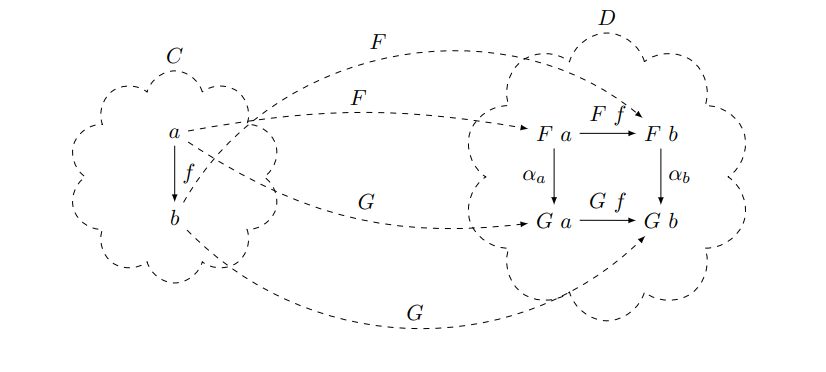
\includegraphics[scale=1.0]{Natural Transformation.png}
\end{center}
\end{definition}

\begin{definition}[Isomorphism]
An isomorphism is a category $\mc{C}$ is a morphism $f:a\to b$ in $\mc{C}$ such that there exists a morphism $f^{-1}:b\to a$ in $\mc{C}$ such that $f^{-1}\circ f=\Id_a:a\to a$ and $f\circ f^{-1}=\Id_b:b\to b$.
\end{definition}

\begin{definition}[Natural isomorphism]
A natural isomorphism is a natural transformation $\a:F\Rightarrow G$ for which each component $\a_x$ is an isomorphism.
\end{definition}

\begin{definition}[Functor category]
The functor category $\mc{D}^\mc{C}$ consists of functors $F:\mc{C}\to\mc{D}$ as objects and natural transformations $\a:F\Rightarrow G$ as morphisms.
\end{definition}

\begin{definition}[Diagram]
When $\mc{C}$ is small, an object $F:\mc{C}\to\mc{D}$ of the functor category $\mc{D}^\mc{C}$ is called a diagram.
\end{definition}

A directed poset $\Lambda$ constitutes a small category, so we can consider diagrams $F:\Lambda\to\mc{D}$ in $\mc{D}^\Lambda$. In our context, a natural isomorphism $\eta:F\Rightarrow F$ of a diagram $F:\Lambda\to\mc{D}$ consists of component isomorphisms $\eta_\lambda:F(\lambda)=Q_\lambda\to F(\lambda)=Q_\lambda$ such that for any morphism $f:\beta\to\alpha$ in $\Lambda$ we have that
\begin{center}
\begin{tikzcd}
F(\beta)=Q_\beta \arrow[r, "F(f)=\phi_{\a\b}"] \arrow[d, "\eta_\beta"'] & F(\alpha)=Q_\alpha \arrow[d, "\eta_\alpha"] \\
F(\beta)=Q_\beta \arrow[r, "F(f)=\phi_{\alpha\beta}"']                   & F(\a)=Q_\alpha                  
\end{tikzcd}
\end{center}
commutes. We have morphisms $f:\b\to\a$ in the directed poset category $\Lambda$ precisely when $\a\leq\b$.

\newpage

\printbibliography

\end{document}
